% Mémo technique — Personal Finance Tracker (préparation de la soutenance)
% Compilation : python tools/build_latex.py   (ou : latexmk -pdf -outdir=build Memo_Technique.tex)
\documentclass[11pt,a4paper]{article}

\usepackage[T1]{fontenc}
\usepackage[utf8]{inputenc}
\usepackage{lmodern}
\usepackage[french]{babel}
\usepackage[margin=2.2cm,headheight=14pt]{geometry}
\usepackage{microtype}
\usepackage{graphicx}
\usepackage{float}
\usepackage[font=small,labelfont=bf]{caption}
\usepackage{subcaption}
\usepackage{booktabs}
\usepackage{tabularx}
\usepackage{array}
\usepackage{longtable}
\usepackage[table]{xcolor}
\usepackage{amssymb}
\usepackage{listings}
\usepackage{tikz}
\usetikzlibrary{positioning,arrows.meta,fit,backgrounds,calc}
\usepackage[most]{tcolorbox}
\usepackage{fancyhdr}
\usepackage{enumitem}
\usepackage{needspace}
\usepackage[hidelinks]{hyperref}
\usepackage[french]{cleveref}

\graphicspath{{../figures/}}
% Generated by tools/build_latex.py — do not edit by hand.
\newcommand{\StudentNameField}{\underline{\hspace{6cm}}}
\newcommand{\SubmissionDate}{October 1, 2026}
\newcommand{\TestCount}{[tests not run]}
\newcommand{\CoveragePct}{[coverage not measured]}
\newcommand{\SampleCount}{311}
\newcommand{\SampleFirstMonth}{2026-04}
\newcommand{\SampleLastMonth}{2026-09}
\newcommand{\VerPython}{3.11.16}
\newcommand{\VerTkinter}{8.6}
\newcommand{\VerPandas}{3.0.6}
\newcommand{\VerMatplotlib}{3.11.2}
\newcommand{\VerPlotly}{7.1.0}
\newcommand{\VerStreamlit}{1.64.0}
\newcommand{\VerPillow}{12.3.0}
\newcommand{\VerPythonPptx}{1.0.2}
\newcommand{\VerPythonDocx}{1.2.0}
\newcommand{\VerPlaywright}{1.63.0}
\newcommand{\VerRich}{15.0.0}
\newcommand{\VerPytest}{9.1.1}
\newcommand{\VerPytestCov}{7.1.0}
\newcommand{\VerRuff}{0.16.9}

% Shared code-listing style for the report and the memo.
% Code excerpts are extracted from the real source by tools/build_latex.py
% (docs/shared/generated/*.py); they are never copied by hand.
\definecolor{codebg}{HTML}{F6F8FA}
\definecolor{codeframe}{HTML}{D0D7DE}
\definecolor{codecomment}{HTML}{2E7D32}
\definecolor{codekeyword}{HTML}{1565C0}
\definecolor{codestring}{HTML}{A0522D}
\lstdefinestyle{project}{
  language=Python,
  basicstyle=\ttfamily\footnotesize,
  keywordstyle=\color{codekeyword}\bfseries,
  commentstyle=\color{codecomment}\itshape,
  stringstyle=\color{codestring},
  backgroundcolor=\color{codebg},
  frame=single, rulecolor=\color{codeframe},
  framesep=3pt, xleftmargin=4pt, xrightmargin=4pt,
  breaklines=true, breakatwhitespace=true,
  postbreak=\mbox{\textcolor{codeframe}{$\hookrightarrow$}\space},
  columns=fullflexible, keepspaces=true,
  showstringspaces=false, tabsize=4,
  upquote=true,
  aboveskip=4pt, belowskip=4pt,
  % pdflatex + listings cannot read multi-byte UTF-8 characters directly:
  % map every non-ASCII character used in the excerpts to a LaTeX equivalent.
  literate=
    {—}{{---}}1 {–}{{--}}1 {→}{{$\rightarrow$}}1 {·}{{$\cdot$}}1
    {✓}{{\checkmark}}1 {✗}{{$\times$}}1 {█}{{\rule{0.5em}{0.7em}}}1
    {💰}{{\$}}1 {é}{{\'e}}1 {è}{{\`e}}1 {à}{{\`a}}1 {ê}{{\^e}}1 {ç}{{\c{c}}}1
    {⚠}{{!}}1 {…}{{...}}1 {─}{{-}}1
}
\lstset{style=project}

\lstset{style=project}
\renewcommand{\lstlistingname}{Extrait}
\renewcommand{\lstlistlistingname}{Liste des extraits}

\definecolor{accent}{HTML}{1565C0}
\definecolor{muted}{HTML}{5F6B66}
\definecolor{defbg}{HTML}{EEF3FB}
\definecolor{anabg}{HTML}{FFF6E5}
\definecolor{anaframe}{HTML}{EF8C00}
% \NoAutoSpacing : babel-french ne doit pas insérer d'espace avant « : » dans le code.
\newcommand{\code}[1]{{\NoAutoSpacing\texttt{#1}}}
\newcolumntype{Y}{>{\raggedright\arraybackslash}X}
\setlength{\parskip}{4pt}
\setlength{\parindent}{0pt}
\setlist{itemsep=2pt,topsep=3pt,leftmargin=1.3em}

\newtcolorbox{definition}[1][]{colback=defbg, colframe=accent, boxrule=0.5pt, arc=2pt,
  left=6pt, right=6pt, top=3pt, bottom=3pt, fonttitle=\bfseries\small,
  title={Définition simple}, #1}
\newtcolorbox{analogie}[1][]{colback=anabg, colframe=anaframe, boxrule=0.5pt, arc=2pt,
  left=6pt, right=6pt, top=3pt, bottom=3pt, fonttitle=\bfseries\small,
  title={Analogie de la vie courante}, #1}
\newtcolorbox{alerte}[1][]{colback=red!4, colframe=red!60!black, boxrule=0.5pt, arc=2pt,
  left=6pt, right=6pt, top=3pt, bottom=3pt, fonttitle=\bfseries\small,
  title={À retenir pour l'oral}, #1}

\pagestyle{fancy}
\fancyhf{}
\fancyhead[L]{\small\color{muted}Mémo technique --- Personal Finance Tracker}
\fancyhead[R]{\small\color{muted}DATA 333}
\fancyfoot[C]{\small\thepage}
\renewcommand{\headrulewidth}{0.4pt}

\hypersetup{pdftitle={Mémo technique --- Personal Finance Tracker},
            pdfsubject={Préparation de la soutenance DATA 333}}

\begin{document}

% ====================================================================== page de garde
\begin{titlepage}
  \centering
  \vspace*{3cm}
  {\Huge\bfseries\color{accent} Mémo technique\par}
  \vspace{0.4cm}
  {\LARGE Personal Finance Tracker\par}
  \vspace{1cm}
  {\large Comprendre et défendre le projet, du plus simple au plus avancé\par}
  \vspace{2.4cm}
  {\large DATA 333 -- Data Management \& Analysis --- Bellevue College\par}
  \vspace{2cm}
  {\large Student Name: \StudentNameField\par}
  \vspace{0.5cm}
  {\large \SubmissionDate\par}
  \vfill
  {\small\color{muted} Document personnel de préparation. Le code, le rapport et les slides
   sont en anglais ; les noms de fichiers, de fonctions et de classes sont donc cités tels
   quels. Tous les extraits de code sont copiés automatiquement depuis le vrai code
   (\code{tools/build\_latex.py}) et toutes les images sont de vraies captures.\par}
\end{titlepage}

\tableofcontents
\newpage

% ====================================================================== 1
\section{Le projet en bref}

\subsection{L'objectif}
Le \emph{Personal Finance Tracker} est une application Python qui sert à suivre son argent :
on y enregistre ses revenus et ses dépenses, on les classe par catégorie, et l'application
transforme ces données en résumés, en tendances, en alertes de budget et en suivi
d'objectifs d'épargne. Elle répond au cahier des charges du cours DATA~333 (suivre revenus et
dépenses, catégoriser, résumer, objectifs d'épargne, fichiers, tendances, graphiques) et
implémente les quatre améliorations demandées : interface Tkinter, stockage JSON \emph{et}
CSV, alertes de budget et tableau de bord Streamlit.

\begin{alerte}
Une phrase pour commencer l'oral : \og Un seul cœur testé (modèles, stockage, analyses,
alertes) et trois façons de s'en servir : la console, une application de bureau et un
tableau de bord web. \fg
\end{alerte}

\subsection{Les fonctionnalités}
\begin{itemize}
  \item \textbf{Transactions} : ajouter, modifier, supprimer, rechercher par texte, filtrer
        (type, catégorie, période, montant). Chaque valeur est vérifiée avant d'être gardée.
  \item \textbf{Résumés et tendances} : revenus, dépenses, solde et taux d'épargne par mois ;
        part de chaque catégorie ; moyenne glissante sur 3 mois ; variation d'un mois à
        l'autre ; plus grosses dépenses.
  \item \textbf{Budgets et alertes} : une limite mensuelle par catégorie ; \emph{WARNING} à
        80\,\%, \emph{EXCEEDED} à 100\,\%, affichée dès qu'une dépense franchit un seuil.
  \item \textbf{Objectifs d'épargne} : montant cible, échéance, versements, jalons à
        25/50/75/100\,\%.
  \item \textbf{Fichiers} : tout l'état en JSON, les transactions en CSV (import/export),
        écriture atomique, récupération d'un fichier corrompu.
  \item \textbf{Graphiques} : camembert par catégorie, barres revenus/dépenses, courbe de
        tendance, progression des objectifs (PNG), plus des graphiques interactifs Plotly.
\end{itemize}

\subsection{Le parcours d'un utilisateur}
\begin{enumerate}
  \item Il lance l'application (console, fenêtre ou navigateur). Au premier lancement, les
        données d'exemple (\SampleCount{} transactions fictives, de \SampleFirstMonth{} à
        \SampleLastMonth) sont chargées pour qu'il ait quelque chose à explorer.
  \item Il ajoute une dépense : type, montant, date, catégorie, description. Une erreur de
        saisie est expliquée et redemandée.
  \item Si la dépense fait dépasser 80\,\% ou 100\,\% d'un budget, une alerte apparaît tout
        de suite.
  \item Il consulte le résumé du mois, la tendance, les graphiques, ses objectifs.
  \item Il quitte : les données sont sauvegardées dans \code{data/my\_finances.json}
        (fichier ignoré par git, pour ne jamais publier de données personnelles).
\end{enumerate}

\subsection{Les trois modes et le tableau de bord}

\paragraph{Mode console --- \code{python main.py cli}.}
Un menu numéroté. Toute la saisie passe par une seule méthode (\code{ConsoleApp.ask}) et des
boucles redemandent la valeur tant qu'elle est invalide (\cref{figm-cli}).

\begin{figure}[H]
  \centering
  \begin{subfigure}[t]{0.49\linewidth}
    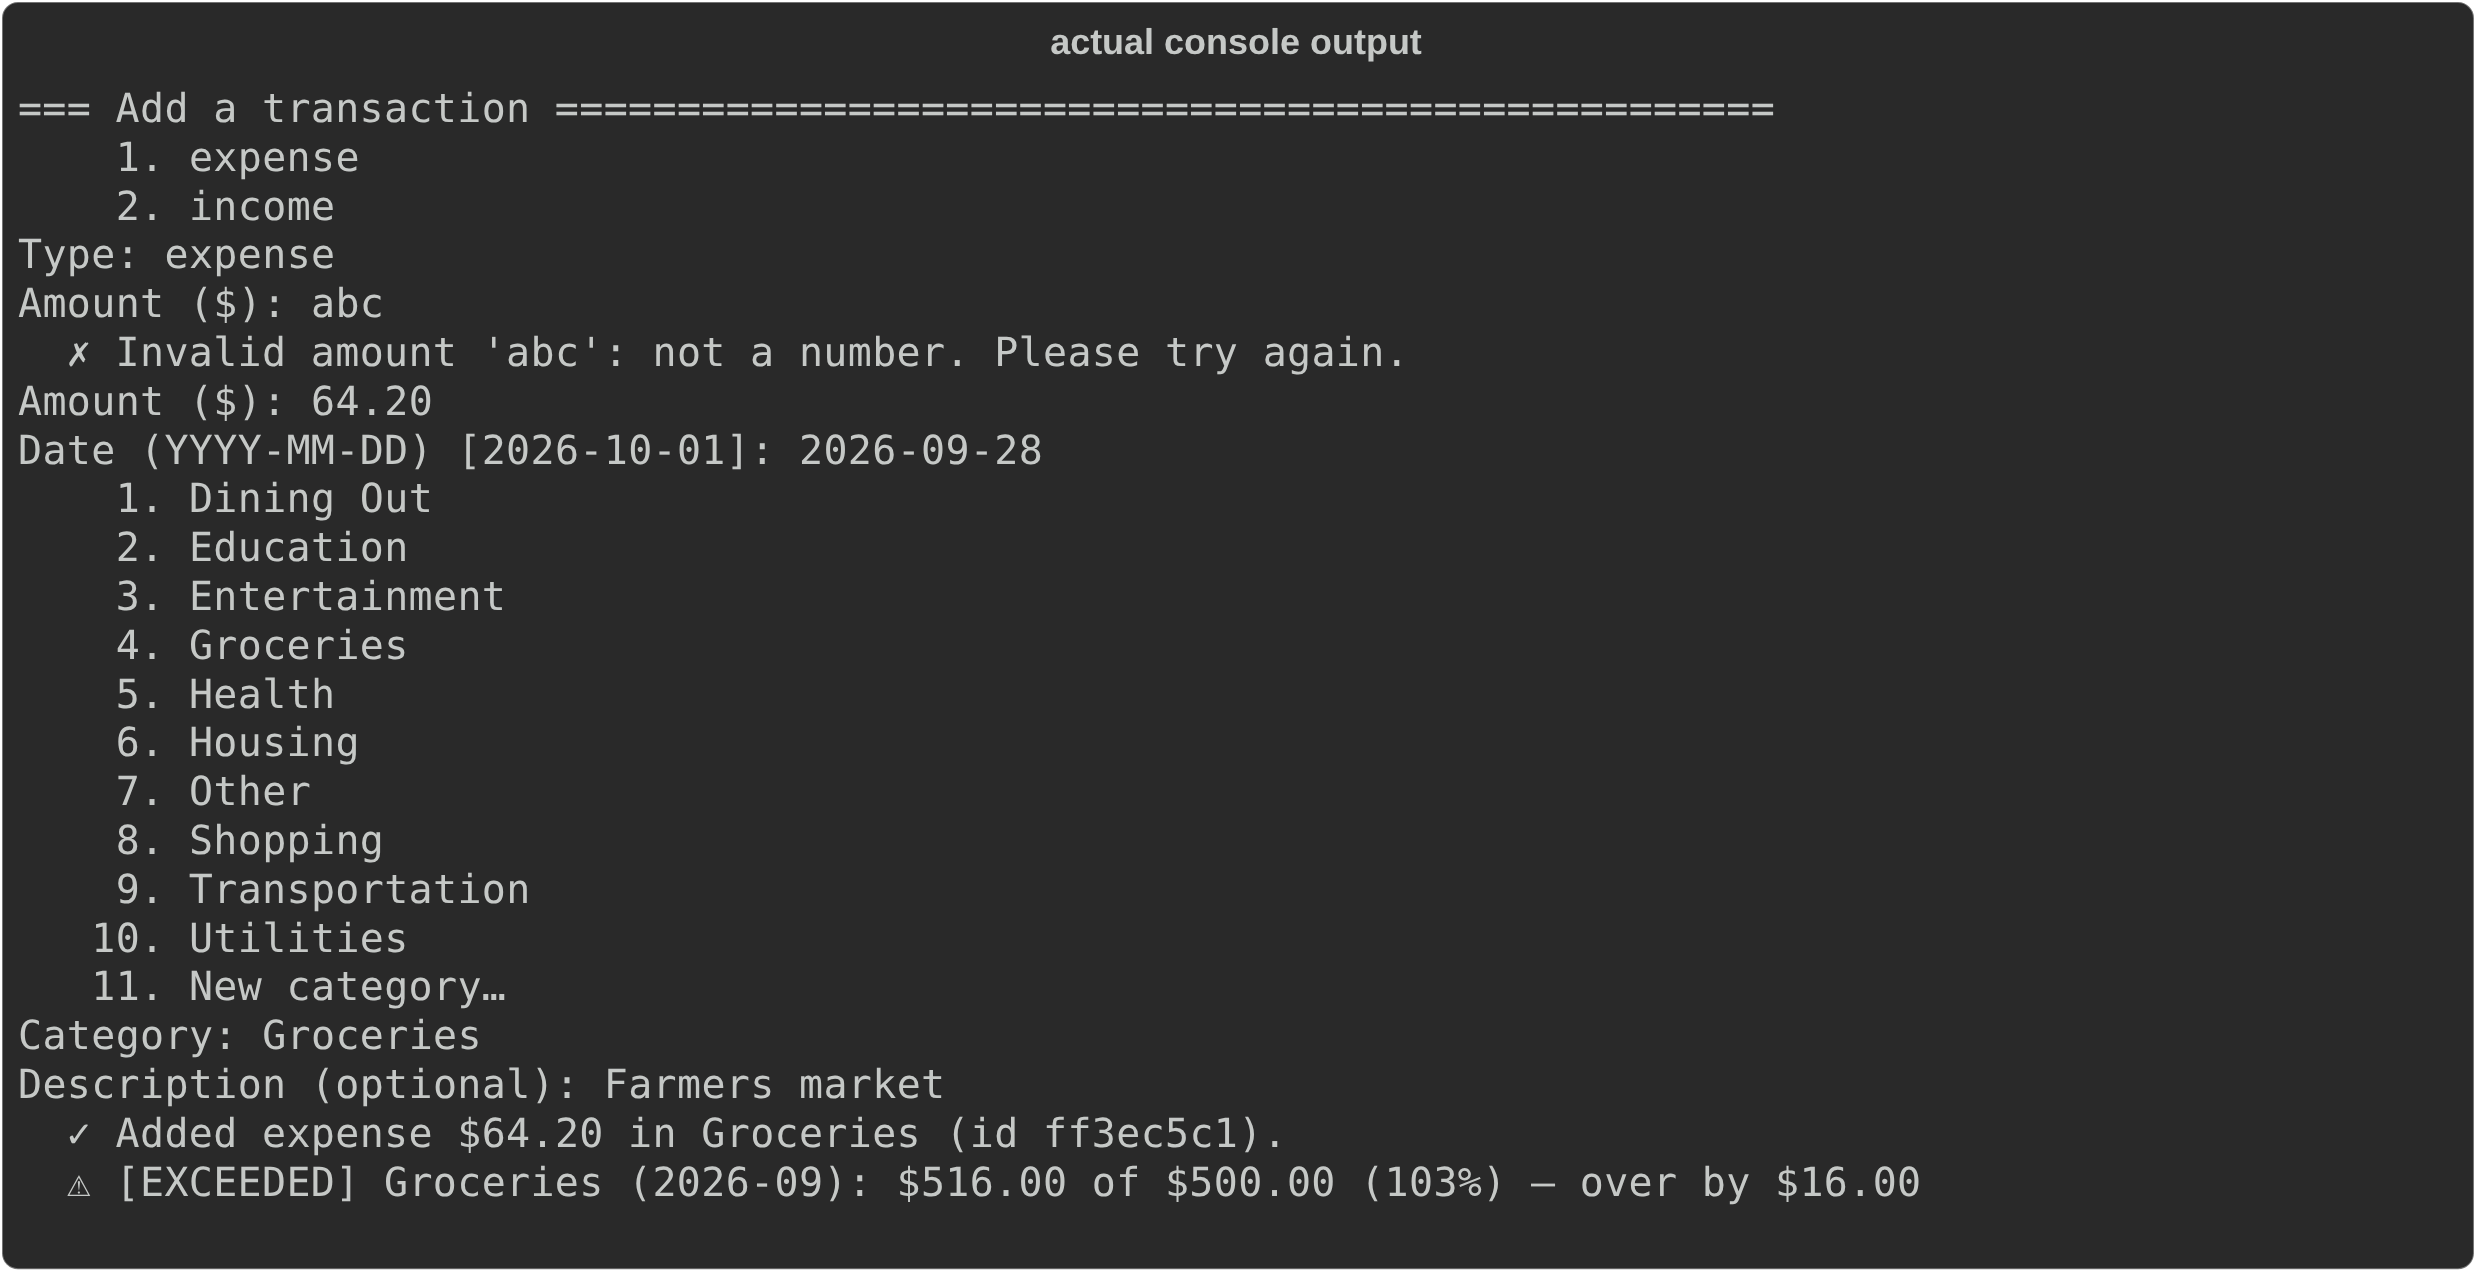
\includegraphics[width=\linewidth]{cli_session_add.png}
    \caption{Ajout d'une dépense : \code{abc} est refusé, puis alerte de budget.}
  \end{subfigure}\hfill
  \begin{subfigure}[t]{0.49\linewidth}
    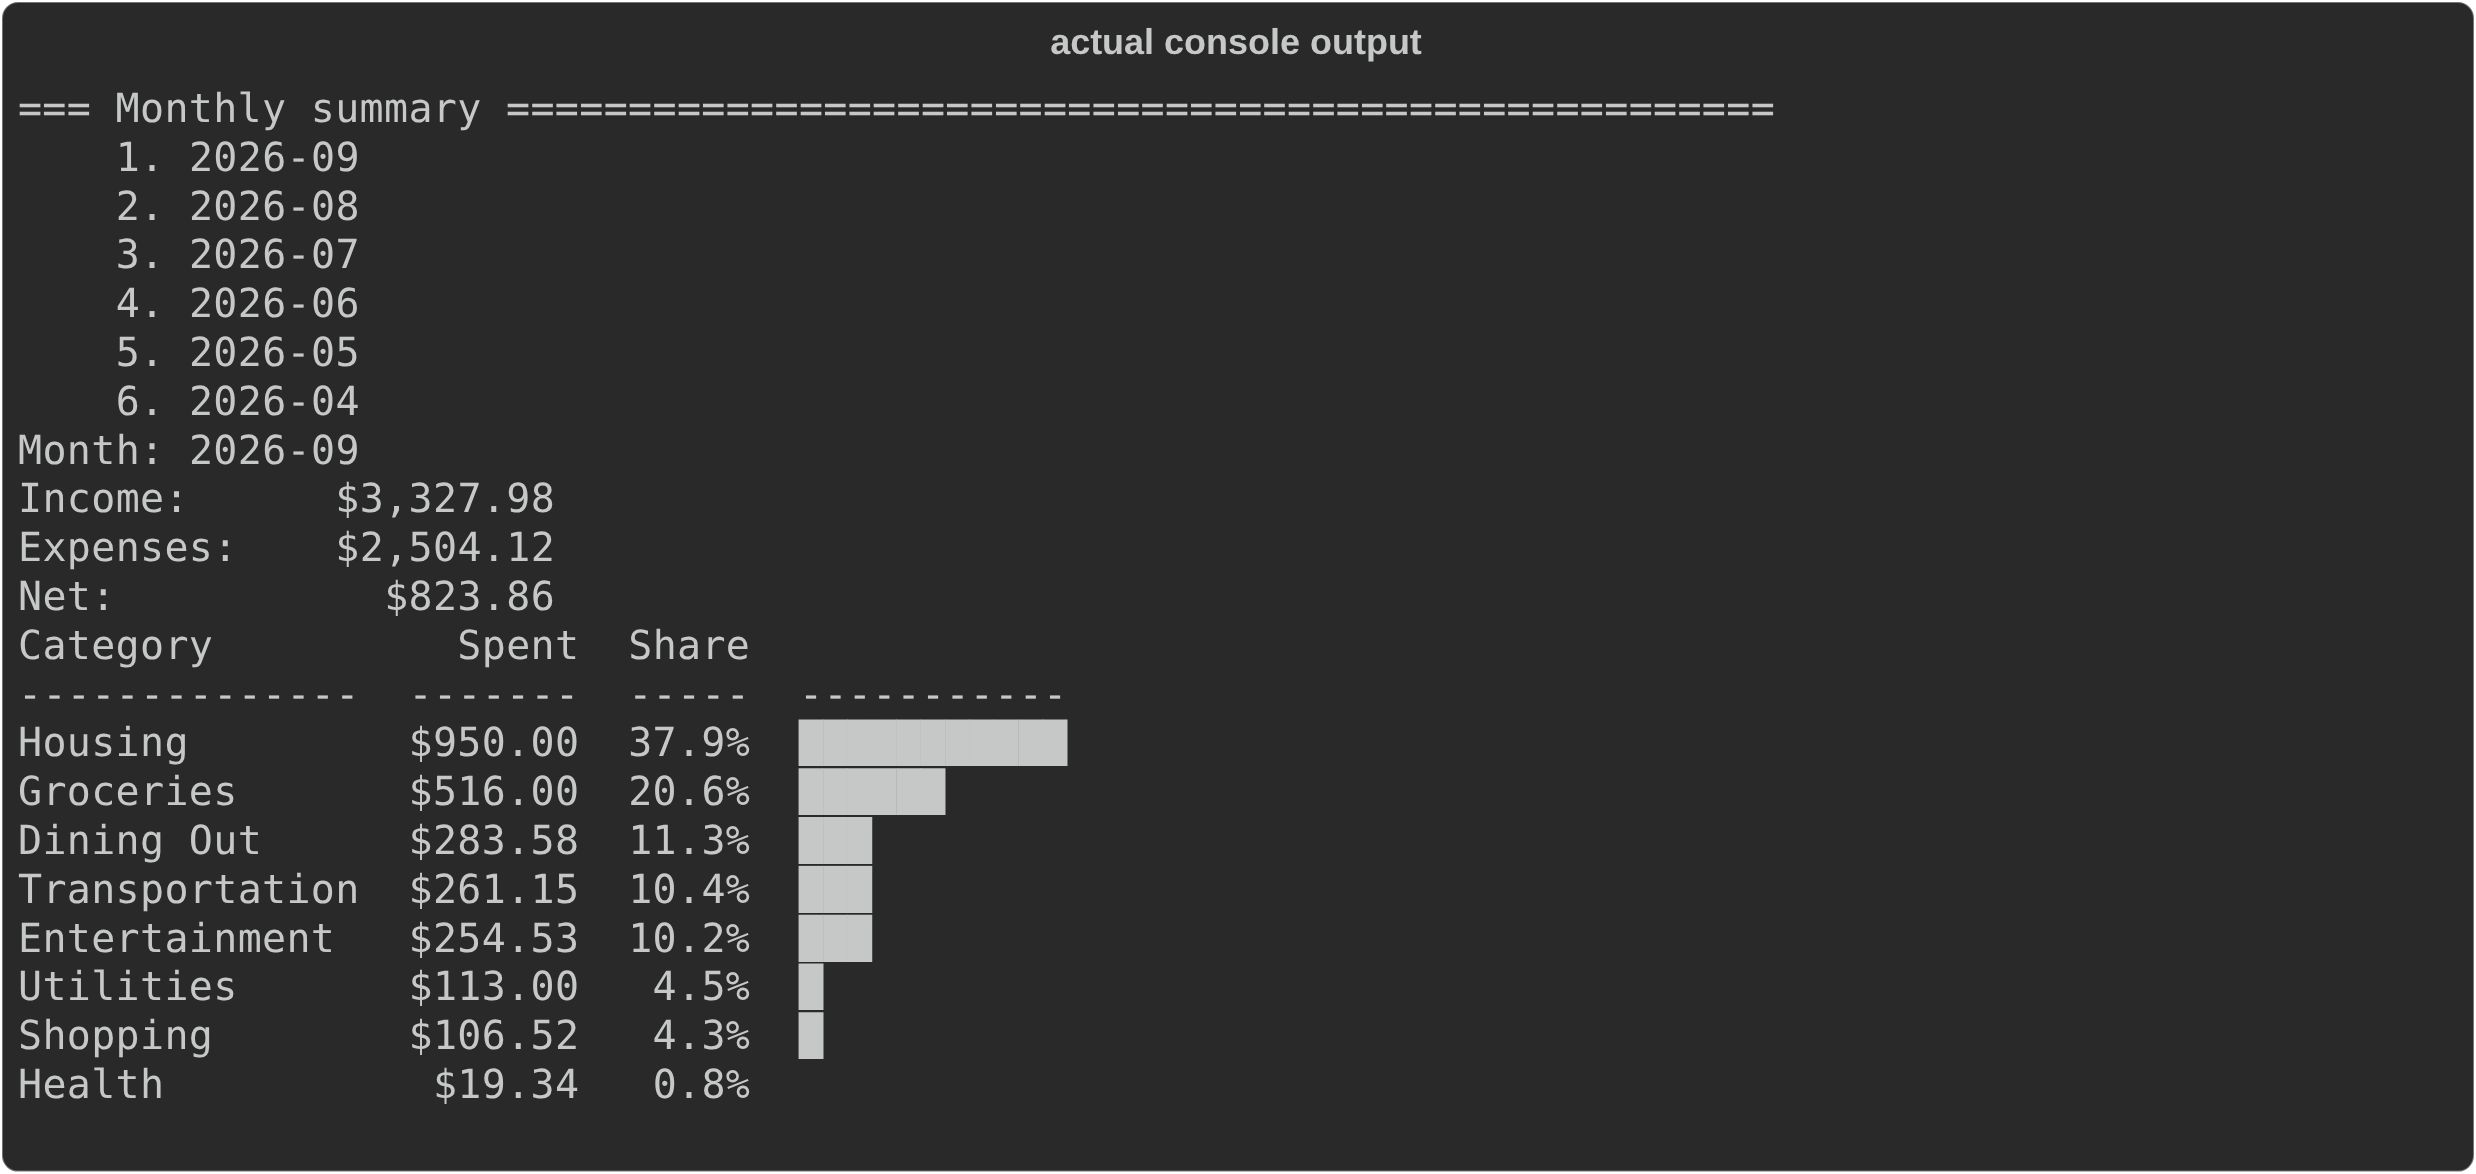
\includegraphics[width=\linewidth]{cli_session_summary.png}
    \caption{Résumé du mois avec la part de chaque catégorie.}
  \end{subfigure}
  \caption{Mode console --- sortie réelle (\emph{actual console output}) d'une session
  \code{python main.py cli} dont les réponses ont été tapées dans un pseudo-terminal.}
  \label{figm-cli}
\end{figure}

\paragraph{Mode démonstration --- \code{python main.py demo}.}
Aucune question : le programme charge les données d'exemple, affiche tous les résumés et
alertes, puis écrit les 4 graphiques PNG et des exports JSON/CSV dans \code{output/}. C'est
le mode à montrer en premier : une seule commande montre tout (\cref{figm-demo}).

\begin{figure}[H]
  \centering
  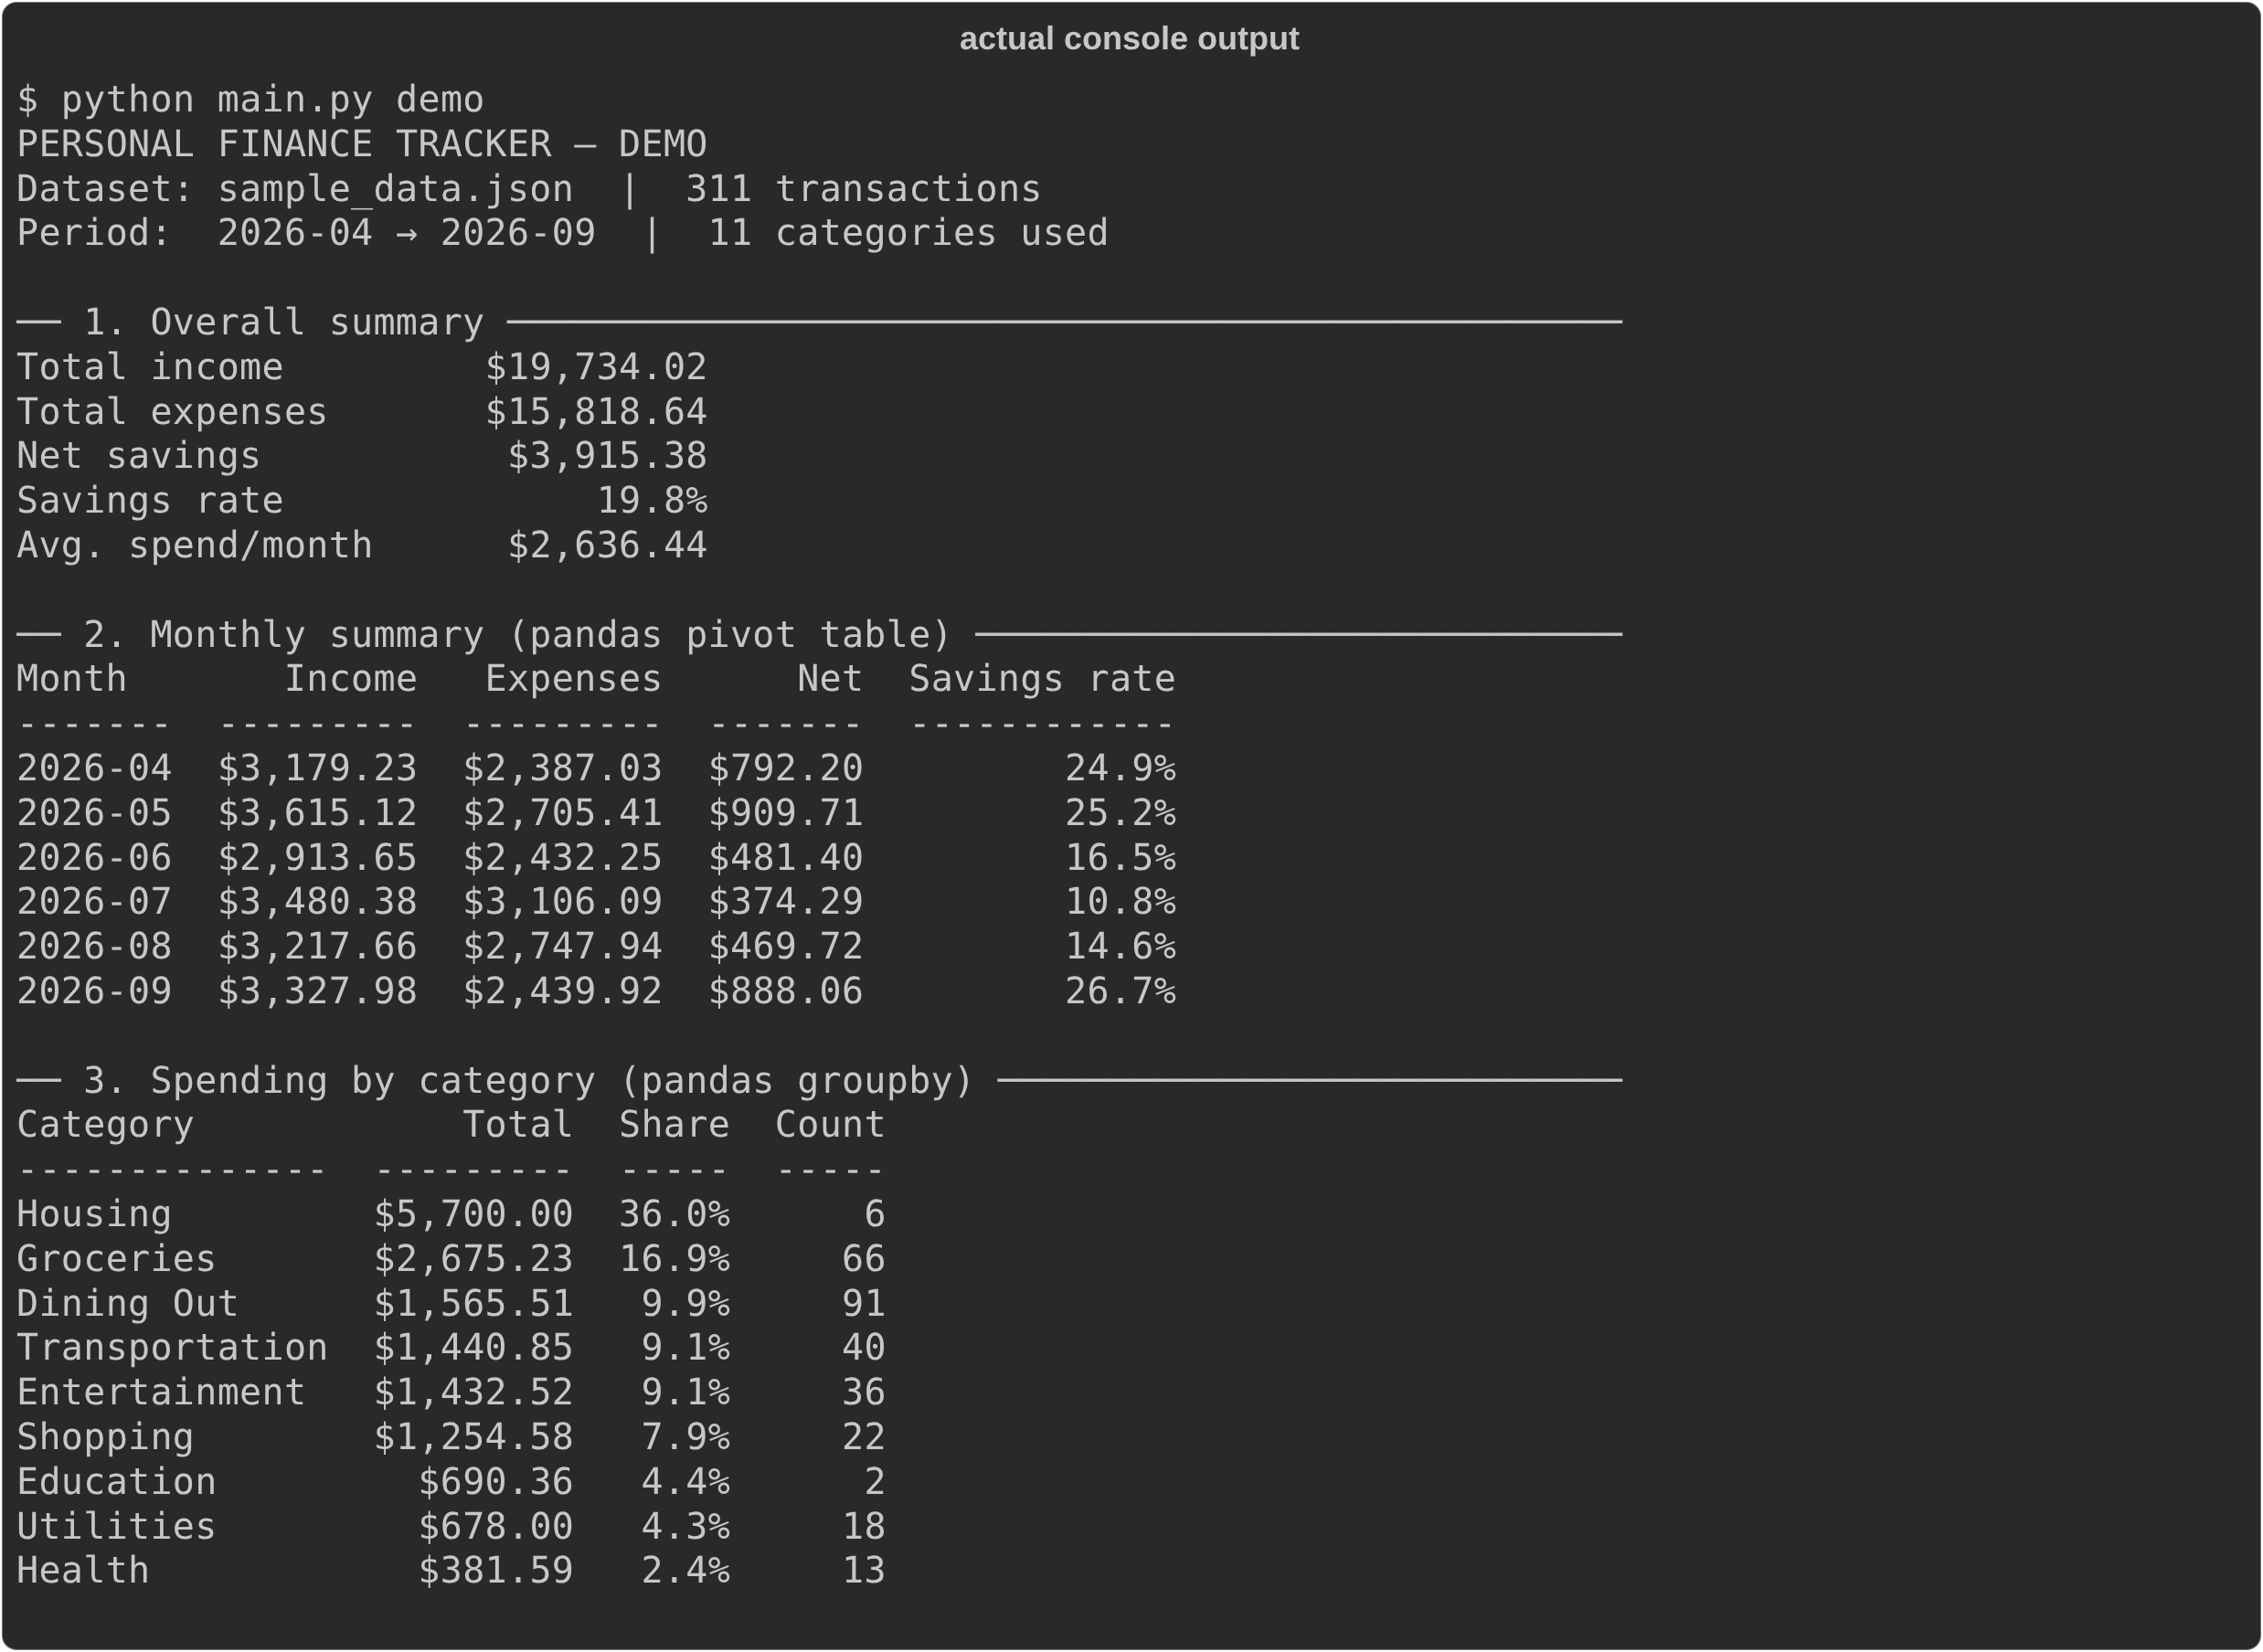
\includegraphics[width=0.78\linewidth]{cli_demo_summary.png}
  \caption{Début de la sortie réelle de \code{python main.py demo} : résumé global, tableau
  mensuel (pandas \code{pivot\_table}) et dépenses par catégorie (\code{groupby}).}
  \label{figm-demo}
\end{figure}

\paragraph{Mode fenêtre --- \code{python main.py gui}.}
Une application Tkinter à quatre onglets : Transactions, Summary, Charts, Budgets \& Goals
(\cref{figm-gui1,figm-gui2}).

\begin{figure}[H]
  \centering
  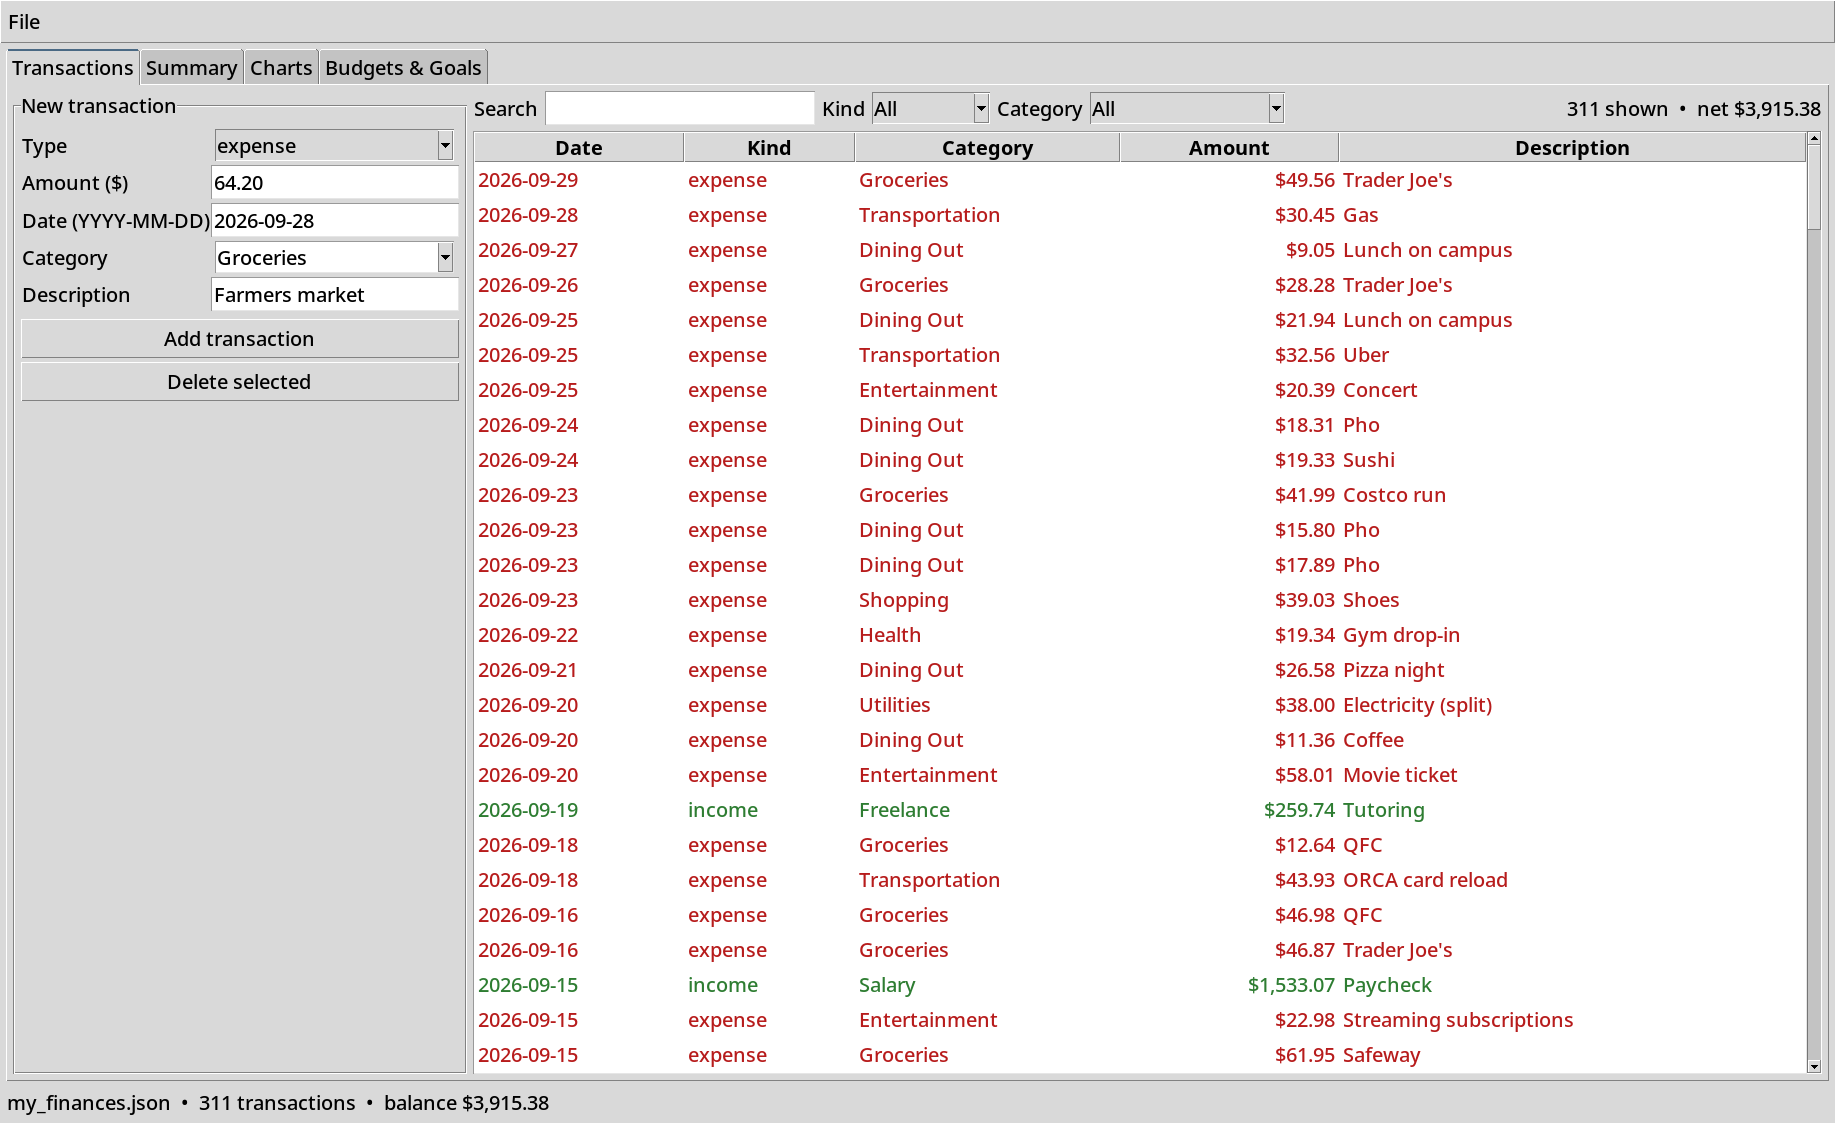
\includegraphics[width=\linewidth,trim=0 227 0 0,clip]{gui_add_form.png}
  \caption{Onglet Transactions : formulaire d'ajout rempli (à gauche), recherche et filtres
  (en haut), tableau triable par colonne. Revenus en vert, dépenses en rouge.}
  \label{figm-gui1}
\end{figure}

\begin{figure}[H]
  \centering
  \begin{subfigure}[t]{0.49\linewidth}
    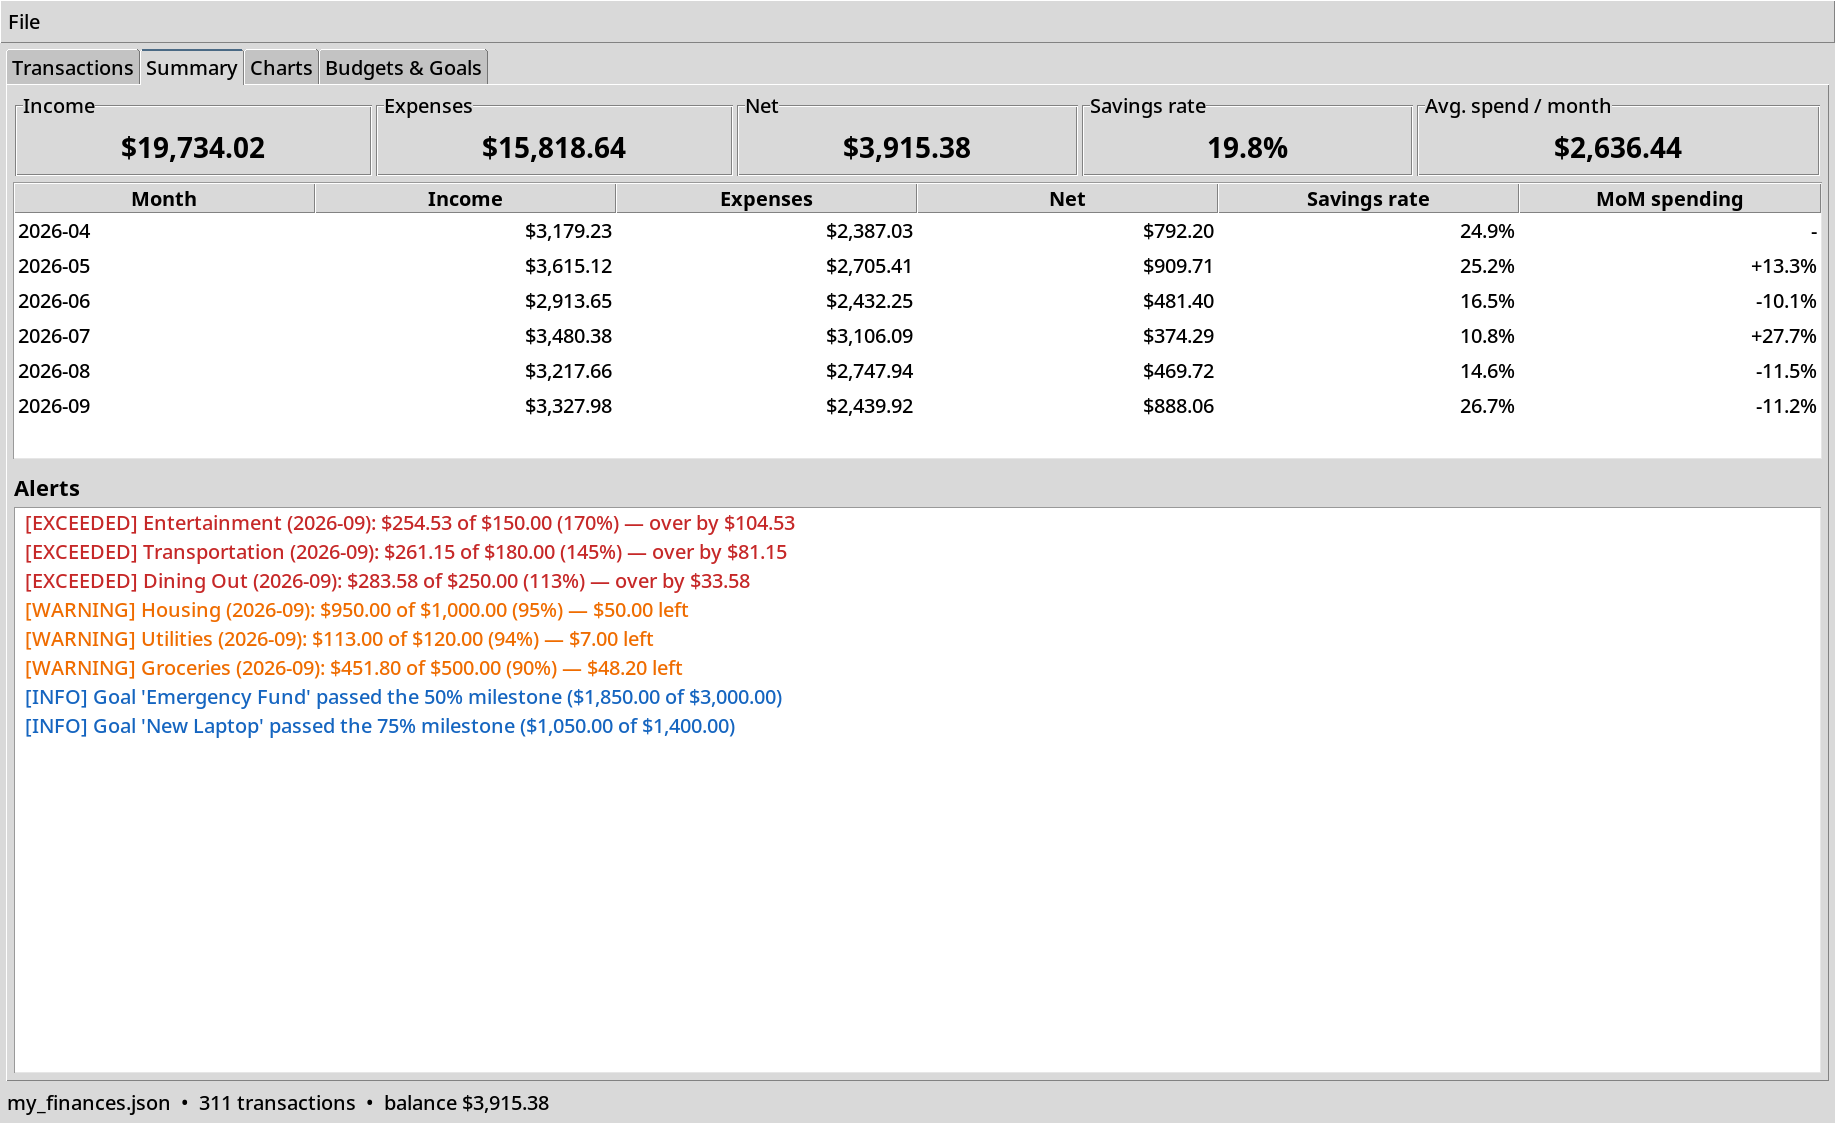
\includegraphics[width=\linewidth,trim=0 240 0 0,clip]{gui_summary.png}
    \caption{Summary : indicateurs, tableau mensuel, alertes colorées.}
  \end{subfigure}\hfill
  \begin{subfigure}[t]{0.49\linewidth}
    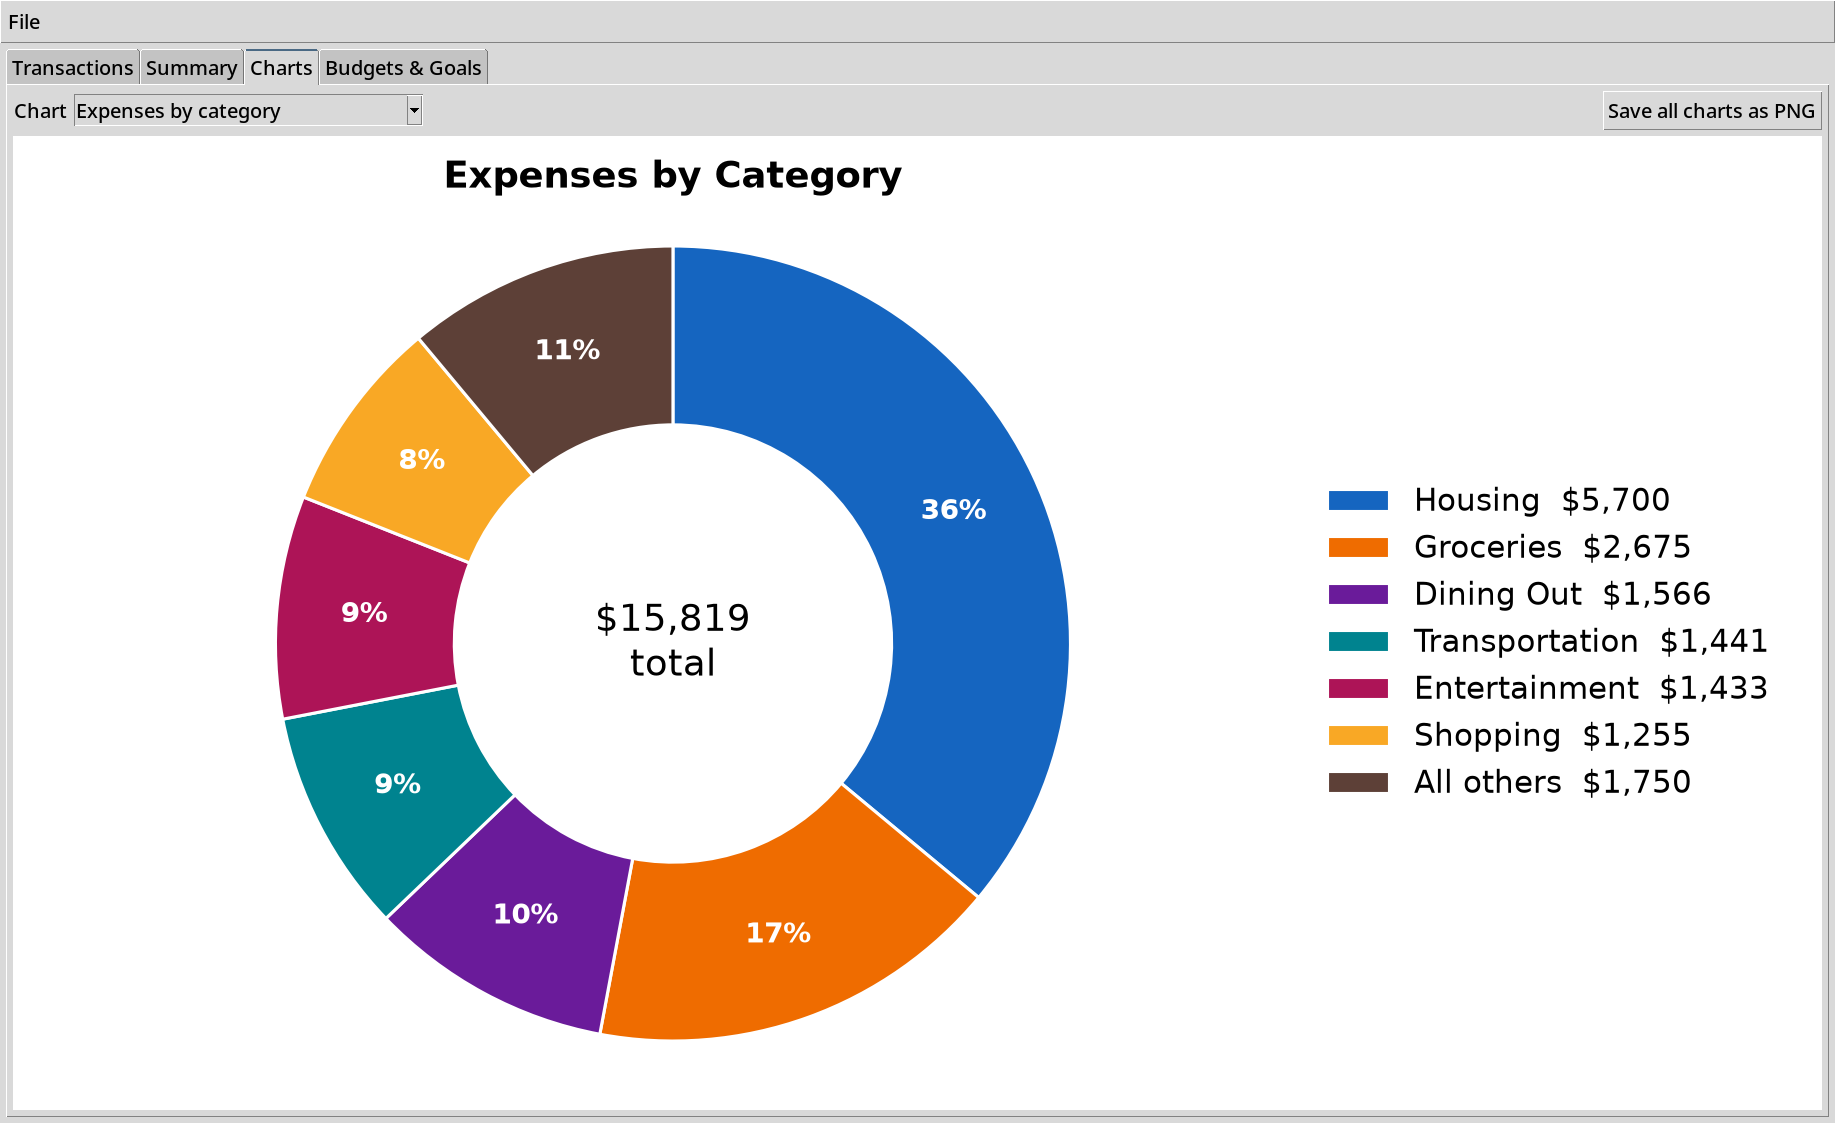
\includegraphics[width=\linewidth]{gui_charts.png}
    \caption{Charts : le même graphique matplotlib que le mode démo.}
  \end{subfigure}

  \medskip
  \begin{subfigure}[t]{0.49\linewidth}
    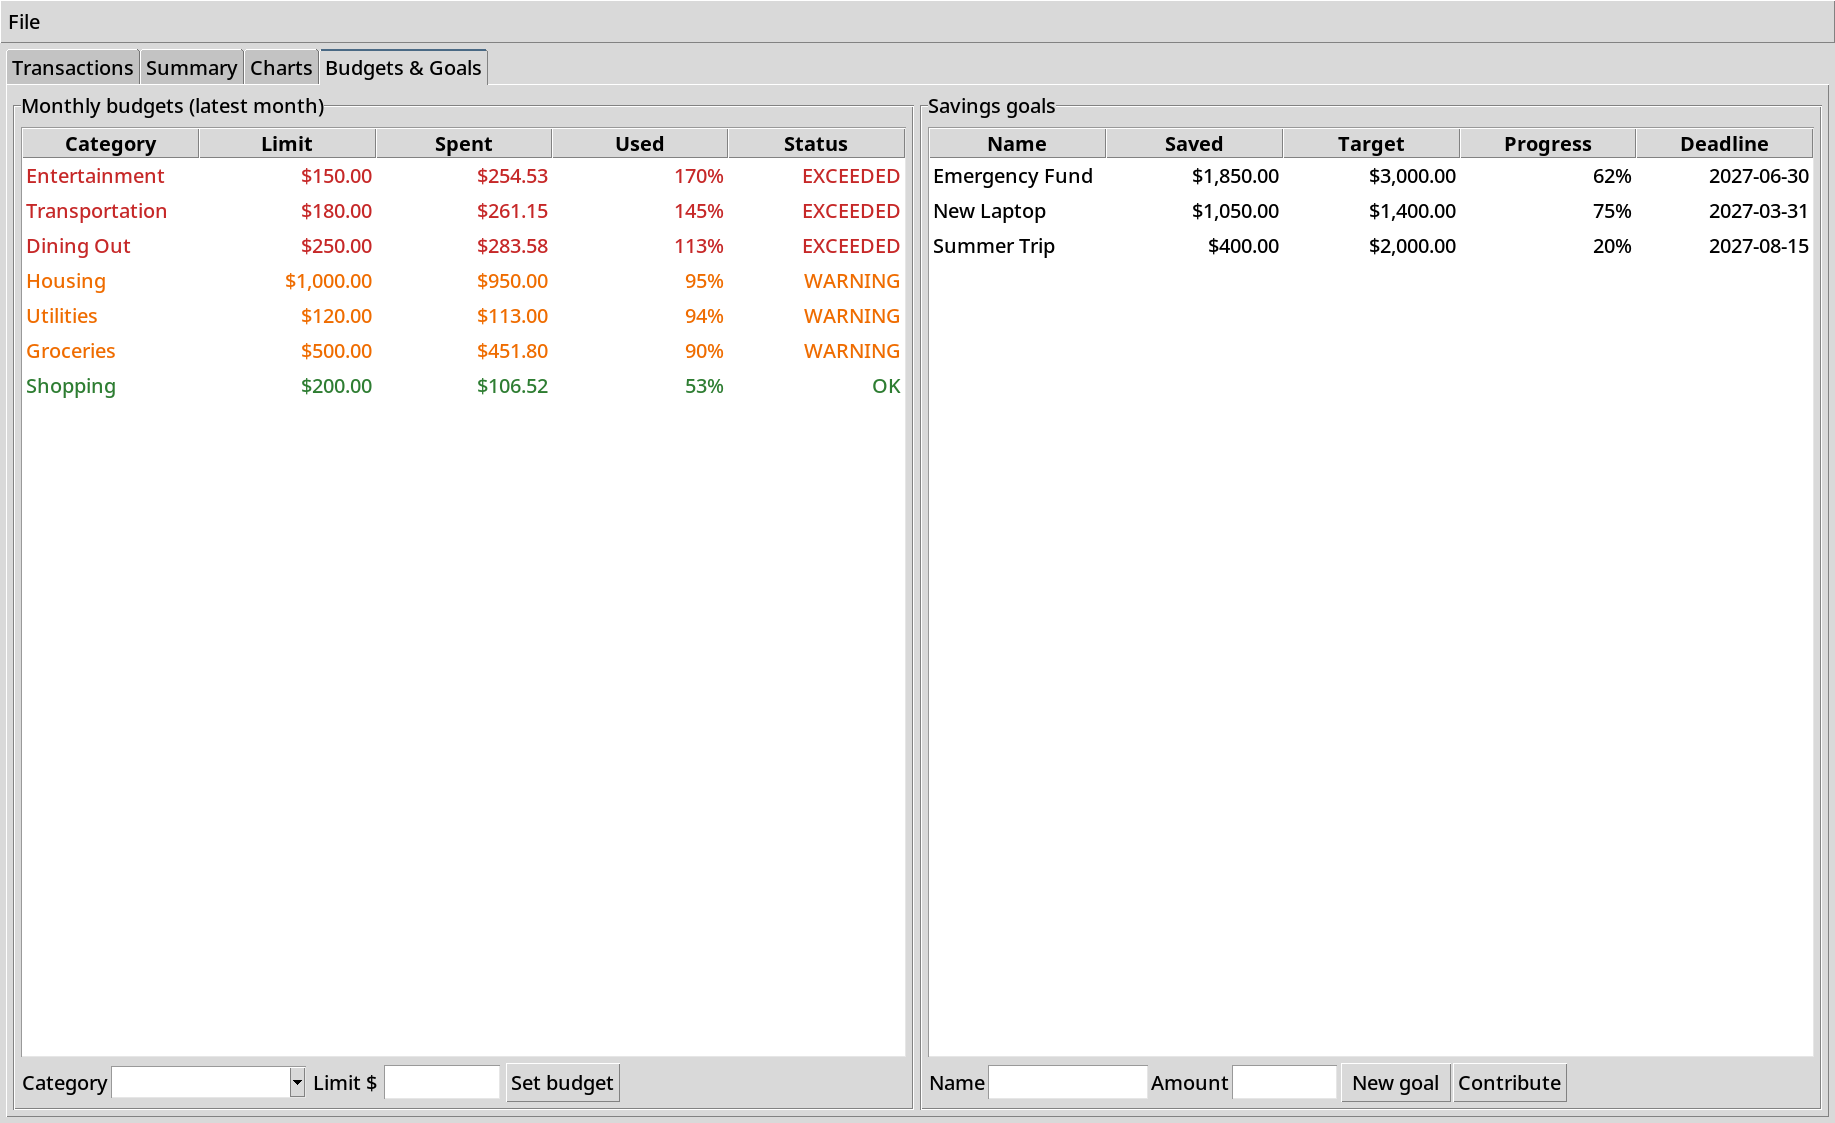
\includegraphics[width=\linewidth,trim=0 313.4 434.4 19.2,clip]{gui_budgets_alerts.png}
    \caption{Budgets : EXCEEDED en rouge, WARNING en orange, OK en vert.}
  \end{subfigure}\hfill
  \begin{subfigure}[t]{0.49\linewidth}
    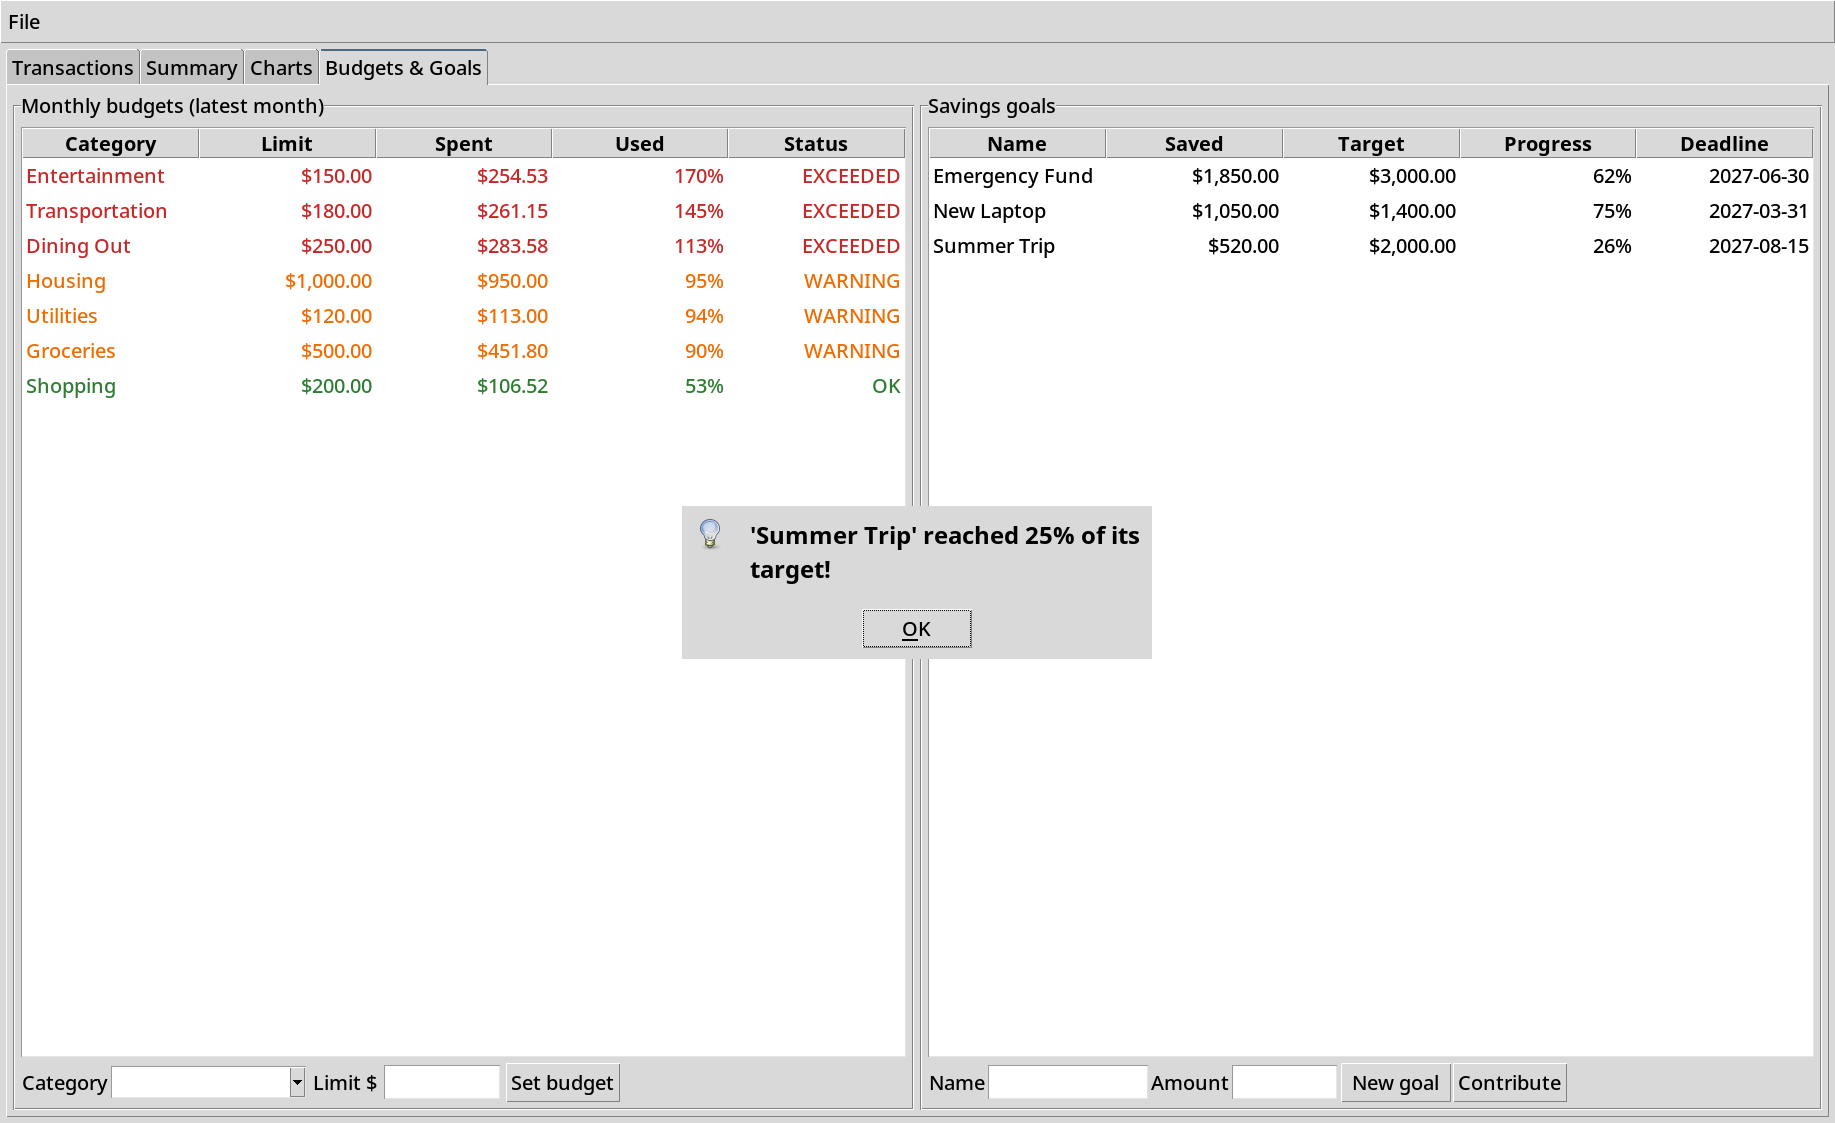
\includegraphics[width=\linewidth,trim=288 212.6 0 19.2,clip]{gui_savings_goals.png}
    \caption{Objectifs : un versement franchit le jalon de 25\,\%.}
  \end{subfigure}
  \caption{Les autres onglets de l'application Tkinter (captures réelles sous Xvfb).}
  \label{figm-gui2}
\end{figure}

\paragraph{Tableau de bord --- \code{streamlit run finance\_tracker/dashboard.py}.}
Une page web interactive : on choisit la source de données (exemple, données sauvegardées ou
fichier importé), on filtre par période, catégories et type, et tout se recalcule
(\cref{figm-dash}).

\begin{figure}[H]
  \centering
  \begin{subfigure}[t]{0.49\linewidth}
    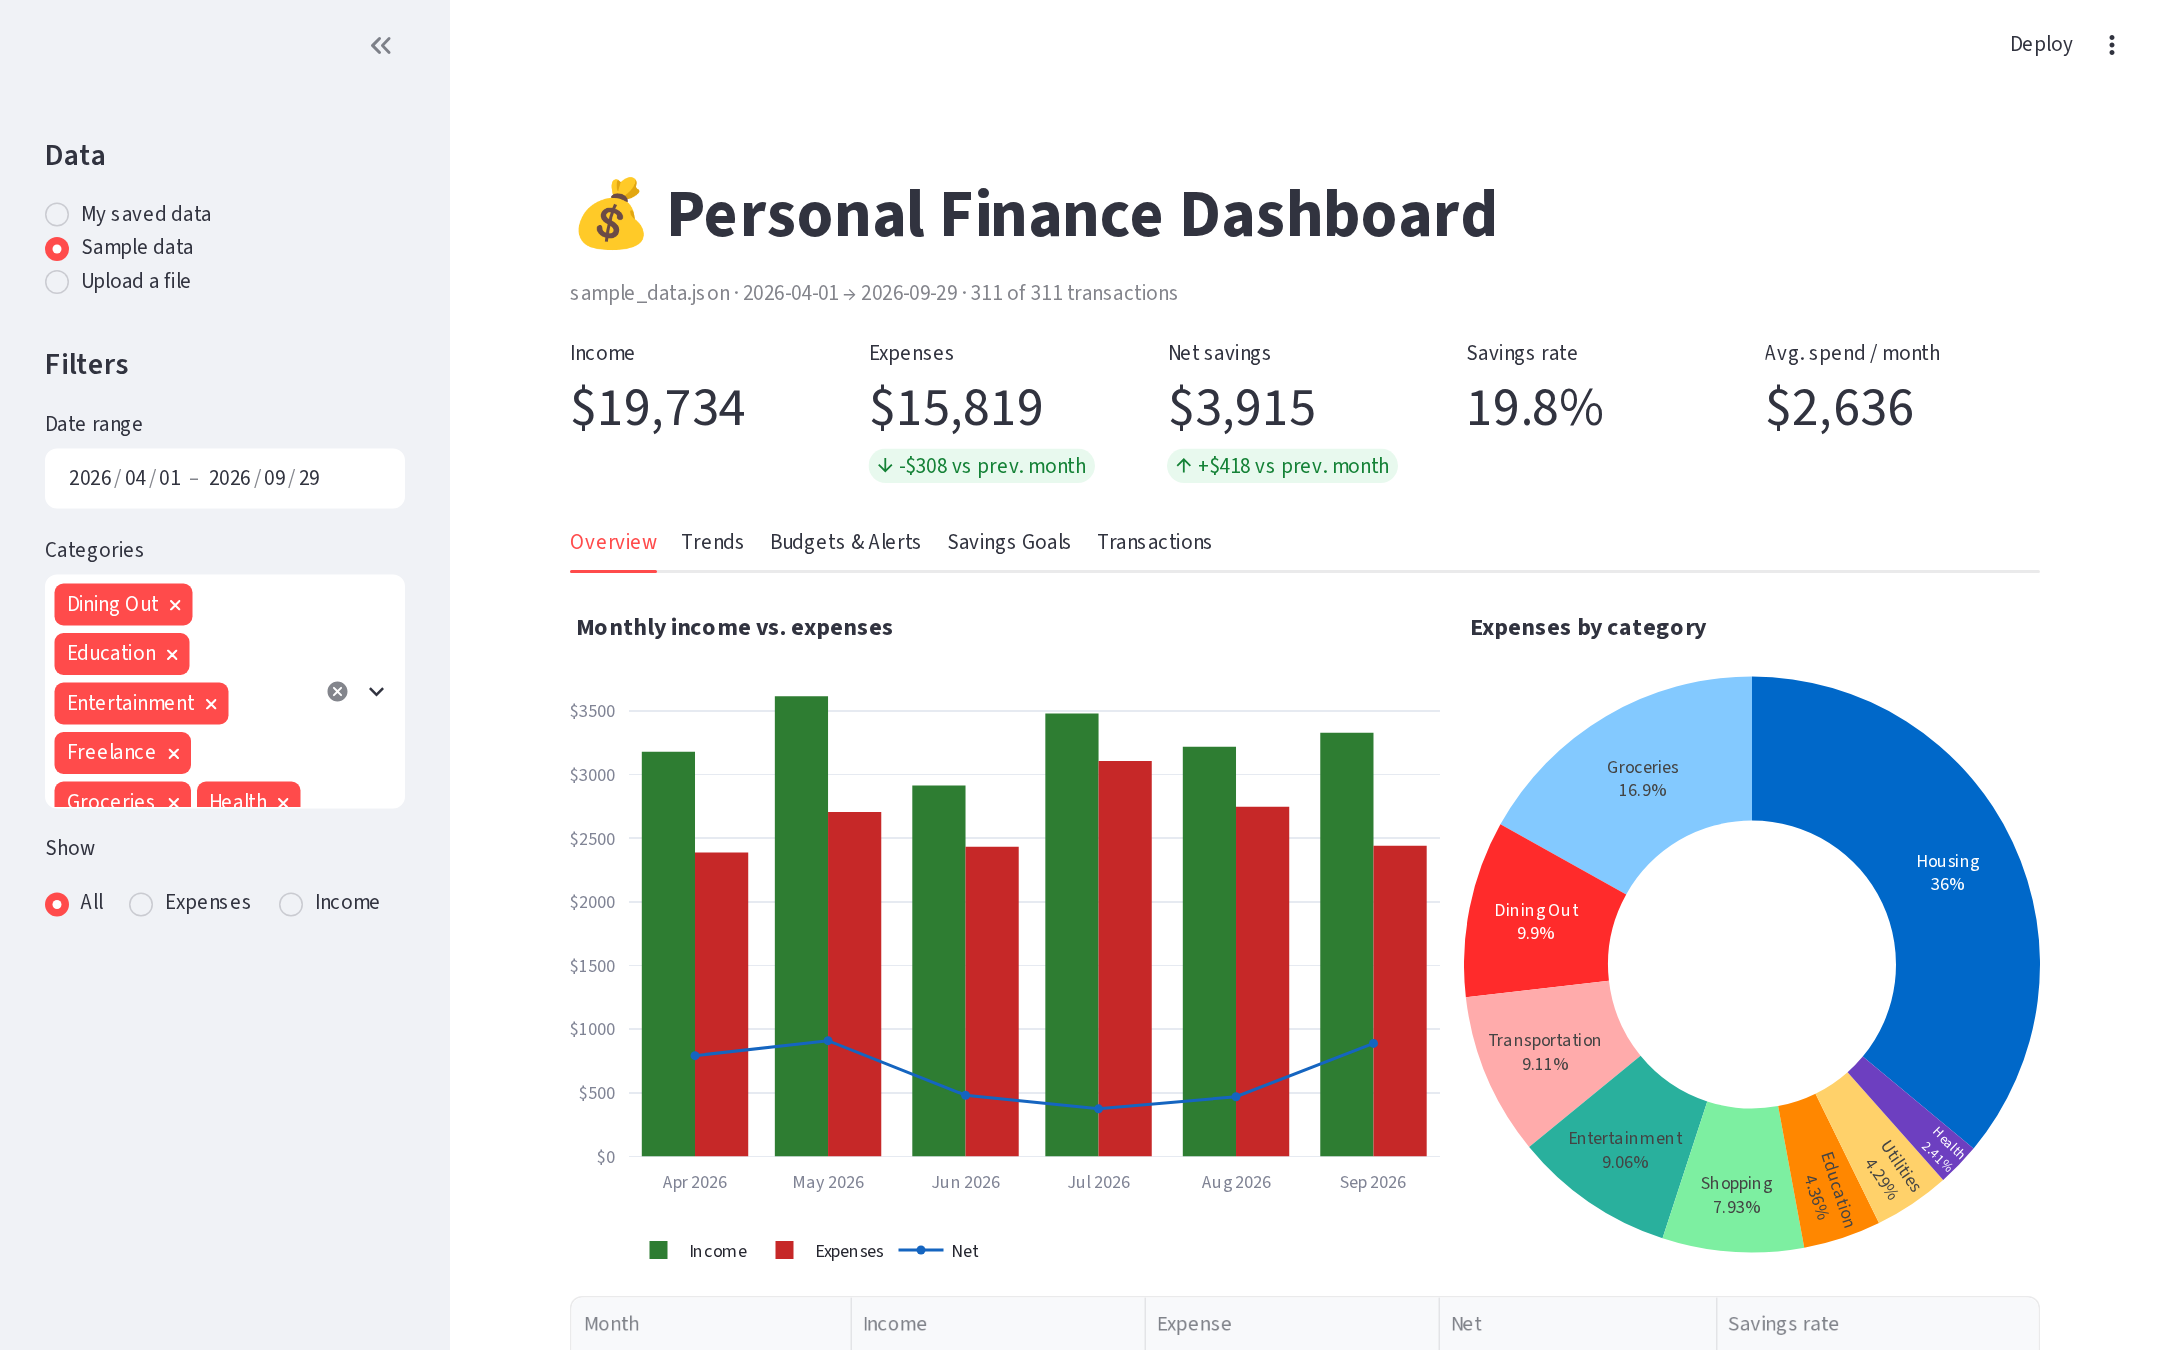
\includegraphics[width=\linewidth]{dashboard_overview.png}
    \caption{Vue d'ensemble : indicateurs et graphiques Plotly.}
  \end{subfigure}\hfill
  \begin{subfigure}[t]{0.49\linewidth}
    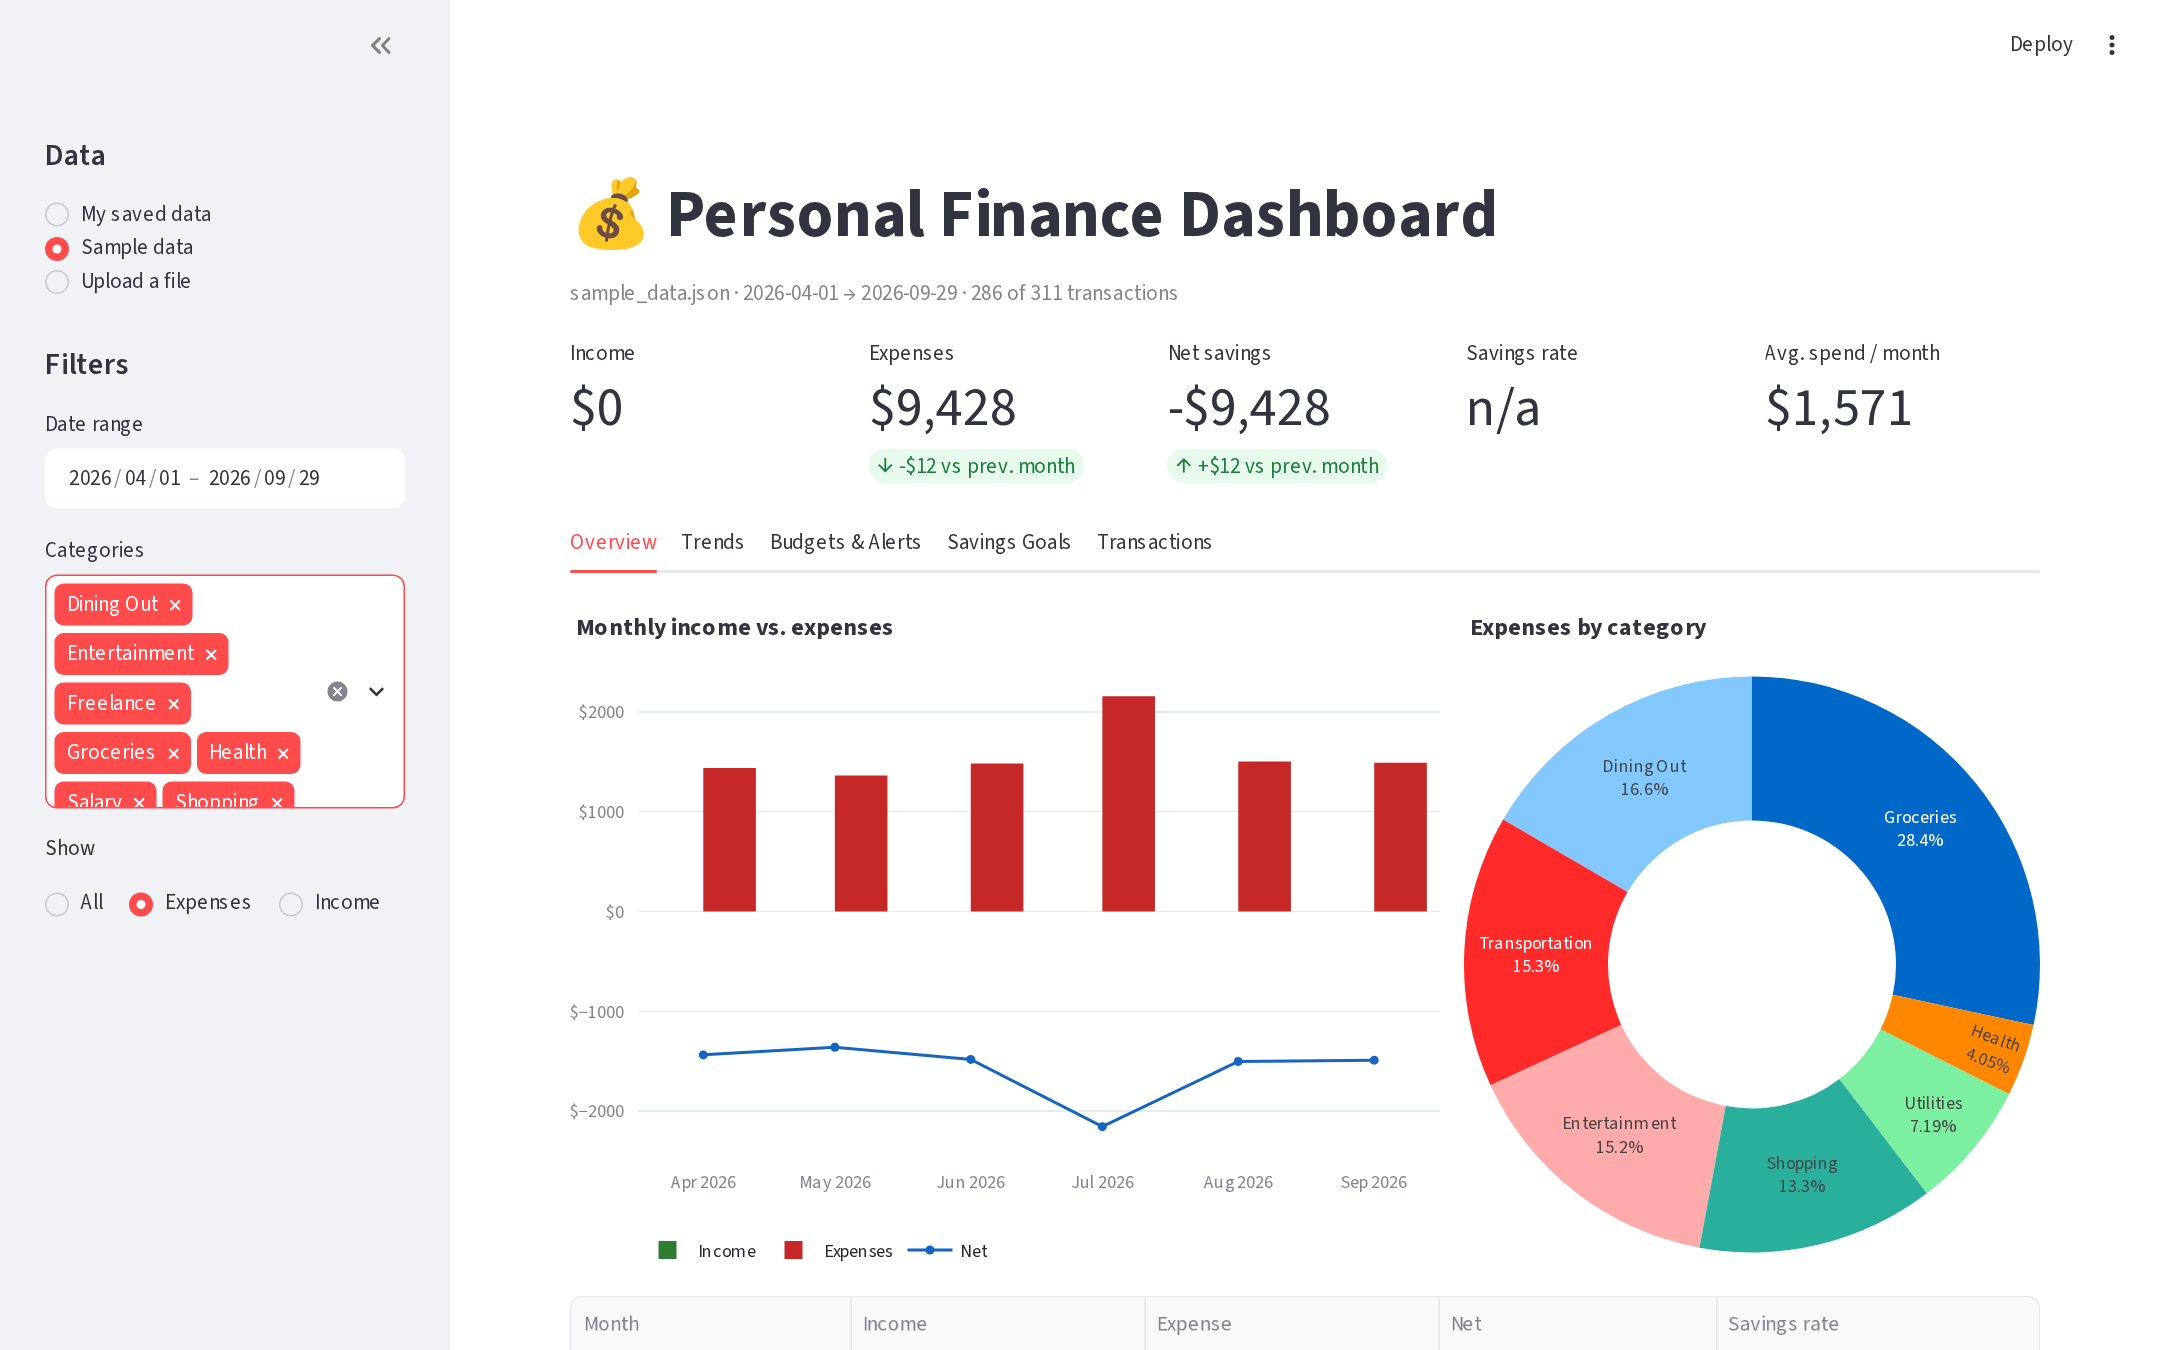
\includegraphics[width=\linewidth]{dashboard_filters.png}
    \caption{Filtres : dépenses seulement, deux catégories retirées.}
  \end{subfigure}

  \medskip
  \begin{subfigure}[t]{0.49\linewidth}
    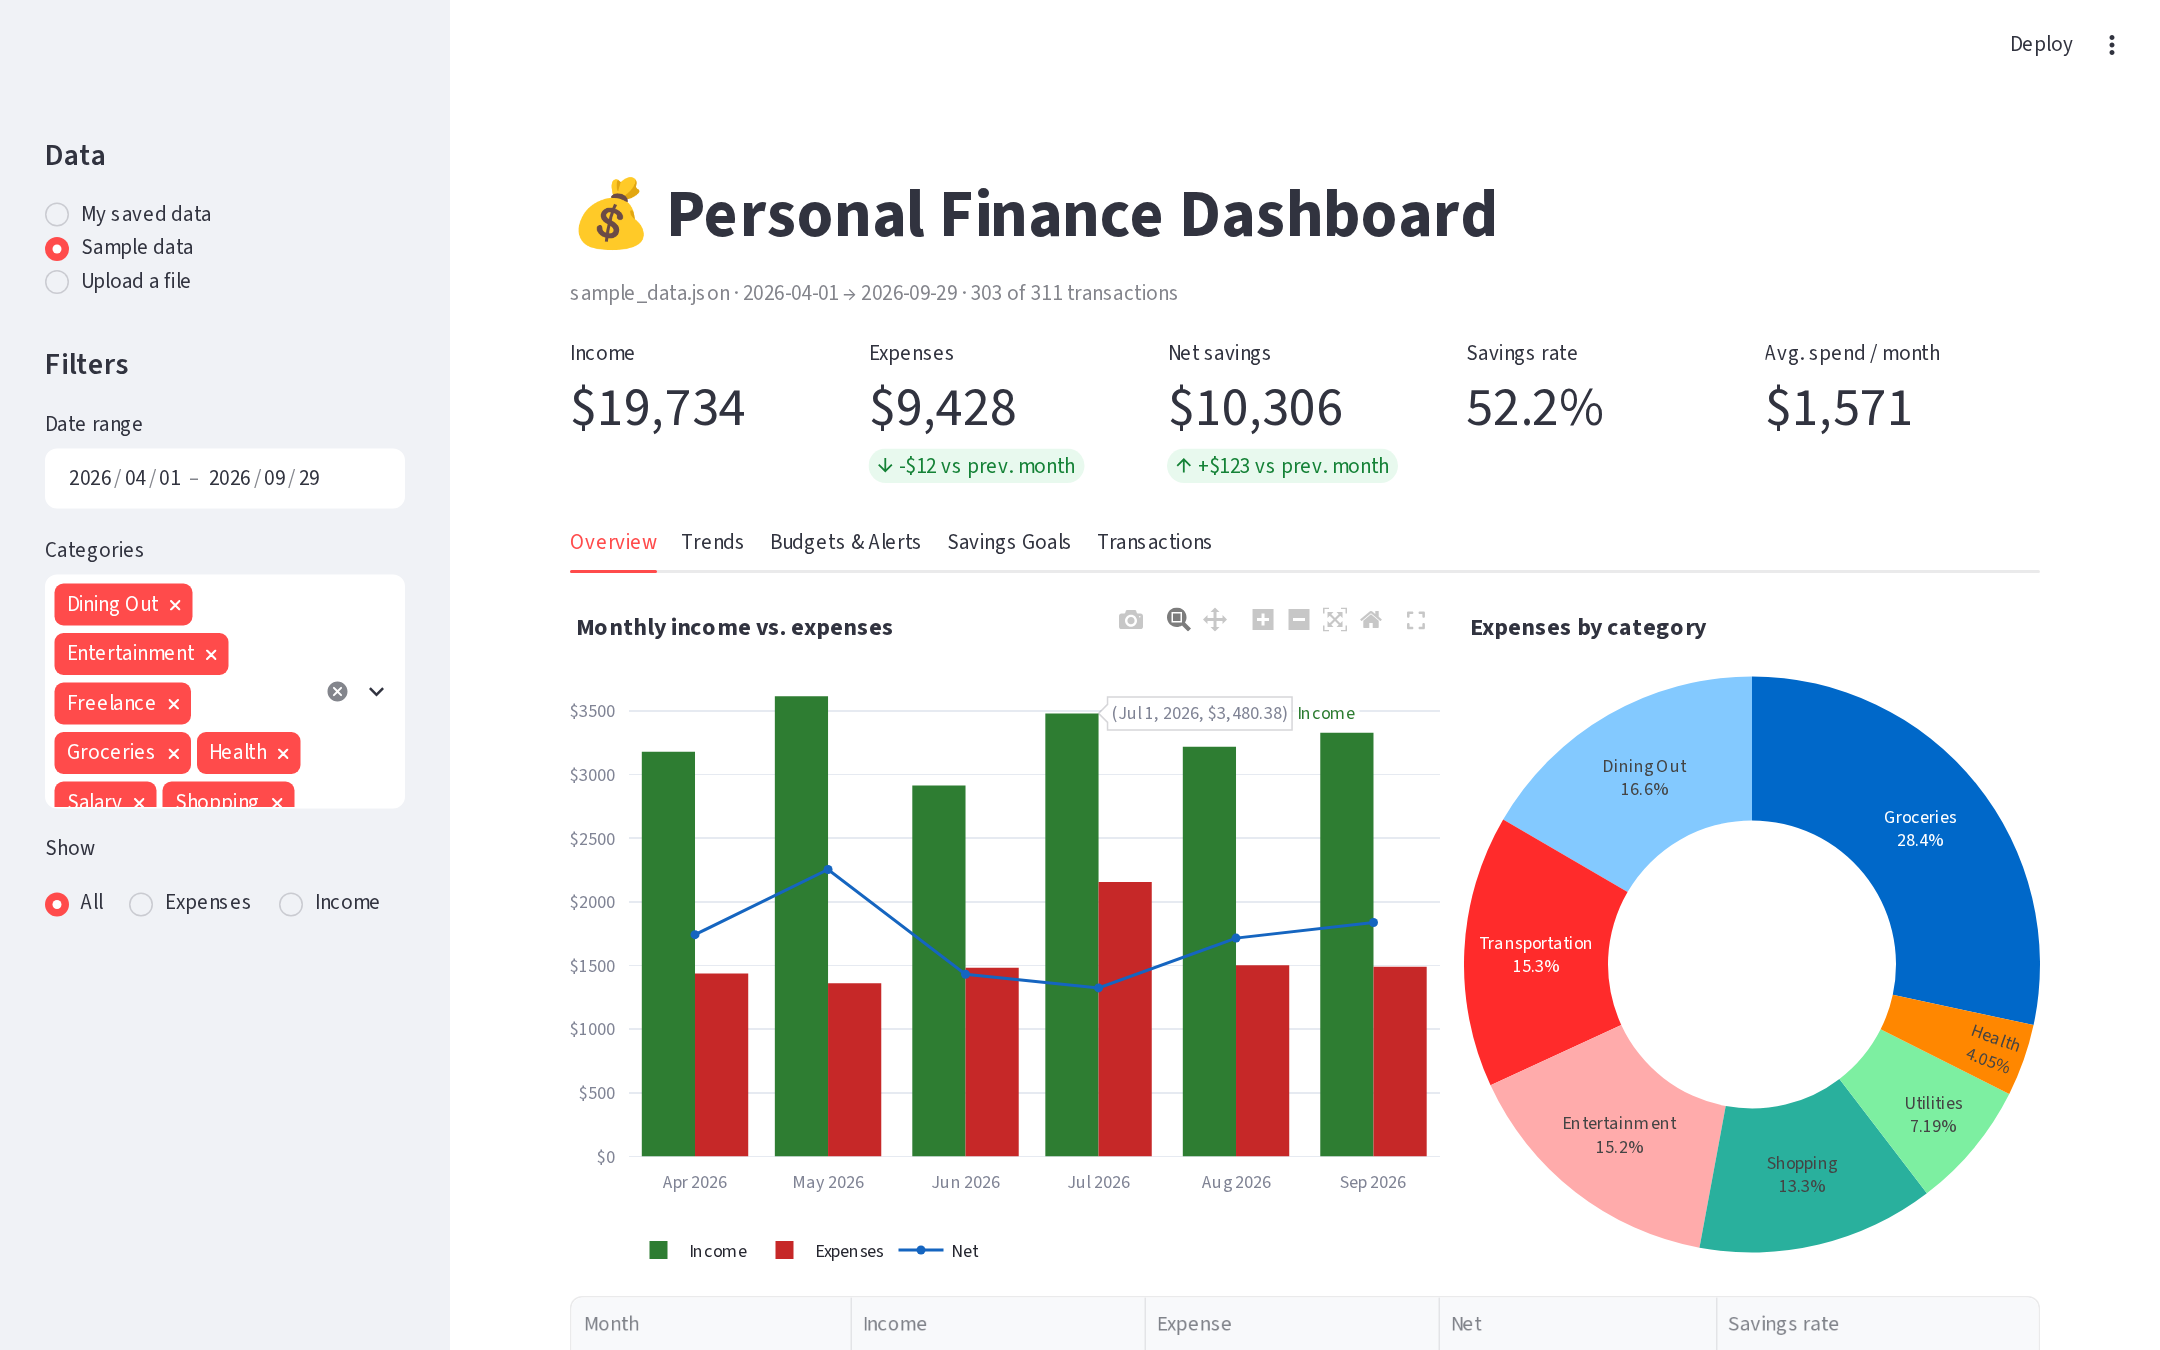
\includegraphics[width=\linewidth]{dashboard_interactive.png}
    \caption{Survol d'une barre : la valeur exacte s'affiche.}
  \end{subfigure}\hfill
  \begin{subfigure}[t]{0.49\linewidth}
    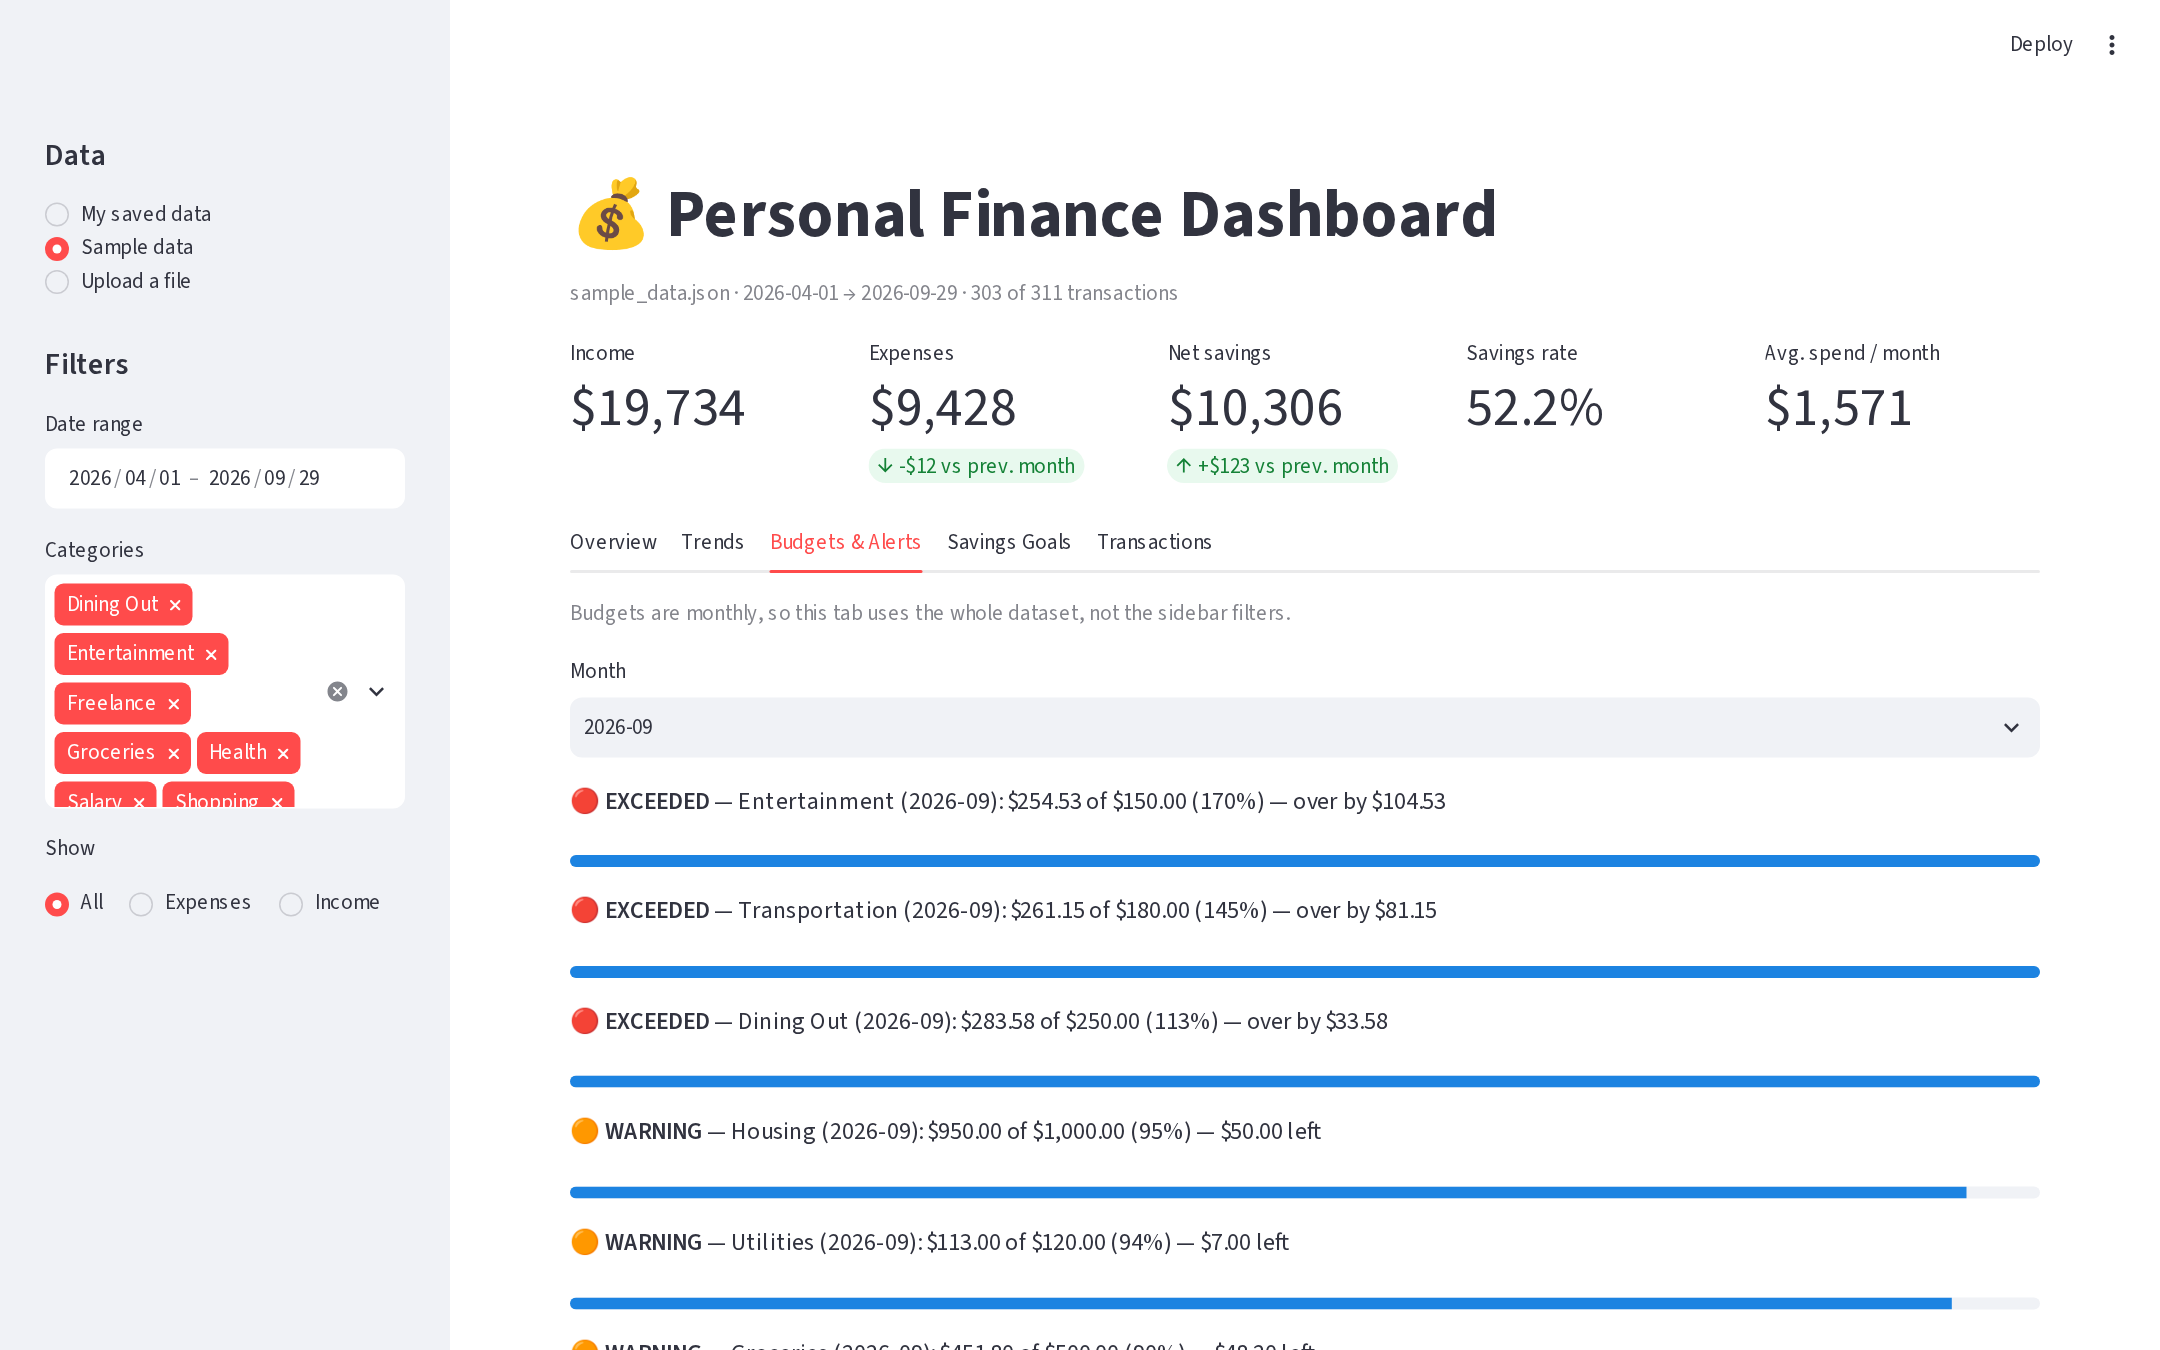
\includegraphics[width=\linewidth]{dashboard_budgets.png}
    \caption{Onglet Budgets \& Alerts.}
  \end{subfigure}
  \caption{Tableau de bord Streamlit, capturé avec Chromium sans affichage (Playwright).}
  \label{figm-dash}
\end{figure}

% ====================================================================== 2
\section{Les concepts du cours, du plus simple au plus avancé}
Pour chaque concept : une définition simple, une analogie, puis l'endroit exact du code où il
est utilisé. Dans le code, chaque concept est marqué par un commentaire \code{\# Concept:}
(\code{grep -rn "\# Concept:" finance\_tracker} les liste tous).

\subsection{Entrées et sorties}
\begin{definition}
Une \emph{entrée} est une information que le programme reçoit (ce que l'utilisateur tape) ;
une \emph{sortie} est ce qu'il affiche ou écrit. En Python : \code{input()} et \code{print()}.
\end{definition}
\begin{analogie}
Un guichet de banque : le client donne une information, le guichetier répond avec un reçu
clair et bien aligné.
\end{analogie}
Dans le projet, \emph{toutes} les lectures clavier passent par \code{ConsoleApp.ask}, et les
fonctions de lecture et d'écriture sont \emph{injectées} dans la classe : les tests peuvent
donc remplacer le clavier par une liste de réponses préparées. Les tableaux sont alignés avec
des f-strings (\code{f"\{montant:>12\}"}).

\subsection{Les décisions (\code{if / elif / else})}
\begin{definition}
Une structure de décision choisit quoi faire selon une condition : \og si \dots{} sinon si
\dots{} sinon \dots{} \fg.
\end{definition}
\begin{analogie}
Un feu tricolore : vert sous 80\,\% du budget, orange entre 80 et 100\,\%, rouge au-delà.
\end{analogie}
\lstinputlisting[caption={\code{alerts.py} --- classer l'utilisation d'un budget}]{../shared/generated/budget_level.py}
Les seuils sont testés du plus grave au moins grave : l'ordre des conditions compte.

\subsection{Les boucles (\code{while}, \code{for})}
\begin{definition}
Une boucle répète des instructions : \code{for} parcourt une collection, \code{while}
recommence tant qu'une condition est vraie.
\end{definition}
\begin{analogie}
Un distributeur de billets qui redemande le code PIN tant qu'il est faux.
\end{analogie}
\lstinputlisting[caption={\code{cli.py} --- redemander le montant tant qu'il est invalide}]{../shared/generated/prompt_amount.py}
Le menu principal est lui aussi une boucle \code{while self.running} ; l'option 0 met
\code{running} à \code{False}.

\subsection{Les fonctions}
\begin{definition}
Une fonction est un bloc de code nommé, qui reçoit des paramètres et renvoie un résultat. On
l'écrit une fois, on l'utilise partout.
\end{definition}
\begin{analogie}
Une recette de cuisine : écrite une fois, réutilisée à chaque repas, avec d'autres
ingrédients.
\end{analogie}
\code{parse\_amount} transforme \code{"\$1,234.50"} en \code{1234.5} et refuse ce qui n'est
pas un montant valable. Elle sert pour les transactions, les budgets \emph{et} les objectifs.
Toutes les fonctions ont des annotations de type et une docstring au format Google
(\code{Args}, \code{Returns}, \code{Raises}), vérifiées par un test.

\subsection{Les listes}
\begin{definition}
Une liste est une collection \emph{ordonnée} d'éléments, qui peut contenir des doublons.
\end{definition}
\begin{analogie}
Un relevé bancaire : les opérations dans l'ordre, et deux cafés identiques peuvent y figurer.
\end{analogie}
\code{FinanceTracker.transactions} est une liste ; les filtres construisent de nouvelles
listes avec des compréhensions de liste.

\subsection{Les dictionnaires}
\begin{definition}
Un dictionnaire associe une \emph{clé} à une \emph{valeur} et retrouve la valeur à partir de
la clé immédiatement.
\end{definition}
\begin{analogie}
Un répertoire téléphonique : on cherche un nom, on obtient le numéro sans lire tout le carnet.
\end{analogie}
Les budgets sont indexés par catégorie, les objectifs par nom, et le menu de la console est un
dictionnaire \og touche $\rightarrow$ (libellé, méthode) \fg : ajouter une option tient en une
ligne.

\subsection{Les ensembles (\code{set})}
\begin{definition}
Un ensemble est une collection \emph{sans doublons} et sans ordre, avec des tests
d'appartenance très rapides.
\end{definition}
\begin{analogie}
Une liste d'invités : ajouter deux fois \og Alice \fg{} ne change rien.
\end{analogie}
\lstinputlisting[caption={\code{tracker.py} --- la liste, les dictionnaires et l'ensemble dans le constructeur}]{../shared/generated/tracker_init.py}
Autre usage : la différence d'ensembles trouve en une expression les colonnes manquantes
d'un CSV (\code{required - set(reader.fieldnames)}).

\subsection{Les classes et la programmation orientée objet}
\begin{definition}
Une classe est un modèle qui regroupe des données (\emph{attributs}) et les actions sur ces
données (\emph{méthodes}). Un objet est un exemplaire construit à partir de ce modèle.
\end{definition}
\begin{analogie}
Le plan d'une maison (la classe) et les maisons construites (les objets), chacune avec ses
pièces et ses usages.
\end{analogie}
Les modèles sont des \emph{dataclasses} : Python écrit le constructeur, et la méthode
\code{\_\_post\_init\_\_} vérifie chaque champ juste après la création. Un objet invalide ne
peut donc jamais exister.
\lstinputlisting[caption={\code{models.py} --- validation d'une transaction à sa création}]{../shared/generated/transaction_post_init.py}

\subsection{La gestion des fichiers}
\begin{definition}
Lire et écrire des fichiers pour que les données survivent à la fermeture du programme.
\end{definition}
\begin{analogie}
Un classeur de bureau : on range les feuilles le soir, on les retrouve le lendemain.
\end{analogie}
\code{storage.py} utilise \code{pathlib} pour les chemins, \code{with open(\dots)} pour être
sûr que le fichier se referme, et les modules \code{json} et \code{csv}. L'écriture est
\emph{atomique} : on écrit d'abord dans un fichier temporaire, puis on le met à la place du
vrai d'un seul coup.
\lstinputlisting[caption={\code{storage.py} --- écriture atomique avec \code{try/except/finally}}]{../shared/generated/atomic_write.py}

\subsection{Les exceptions}
\begin{definition}
Une exception signale une erreur pendant l'exécution. On peut l'\emph{attraper}
(\code{try/except}) pour réagir proprement au lieu de planter.
\end{definition}
\begin{analogie}
L'airbag d'une voiture : quand un problème survient, il amortit le choc au lieu de laisser
tout s'écraser.
\end{analogie}
Le projet définit sa propre hiérarchie d'erreurs : l'interface attrape
\code{FinanceTrackerError} une seule fois et affiche le message, quelle que soit l'erreur
précise.
\lstinputlisting[caption={\code{exceptions.py} --- la hiérarchie complète des erreurs}]{../shared/generated/exceptions_all.py}

\subsection{pandas}
\begin{definition}
pandas manipule des \emph{tableaux de données} (DataFrame) : filtrer, regrouper, agréger,
calculer des moyennes glissantes, en une ligne au lieu d'une boucle.
\end{definition}
\begin{analogie}
Un tableur Excel automatisé : un seul \code{groupby} fait ce qu'on ferait à la main avec des
filtres et des sous-totaux.
\end{analogie}
\lstinputlisting[caption={\code{analytics.py} --- résumé mensuel par tableau croisé}]{../shared/generated/monthly_summary.py}
\code{pivot\_table} met une ligne par mois et une colonne par type (revenu, dépense) ; le
taux d'épargne est protégé contre la division par zéro (\code{where(income > 0)}).

% ====================================================================== 3
\section{Les bibliothèques}
Pour chacune : à quoi elle sert, une analogie, où et comment elle est utilisée, et pourquoi ce
choix plutôt qu'une alternative. Les versions sont celles réellement installées.

\needspace{8\baselineskip}
\subsection{pandas (\VerPandas)}
\textbf{Rôle.} Toutes les analyses : résumé mensuel, catégories, tendance, plus grosses
dépenses, indicateurs. \textbf{Analogie.} Un tableur qui obéit à des formules écrites une
fois. \textbf{Où.} \code{analytics.py}, puis le tableau de bord et la démo.
\lstinputlisting[caption={\code{analytics.py} --- \code{groupby} avec agrégation nommée}]{../shared/generated/category_breakdown.py}
\textbf{Pourquoi pandas.} Le cours l'exige, et des boucles Python feraient le même travail en
trois fois plus de lignes, avec plus de risques d'erreur. NumPy seul n'a pas d'étiquettes
(mois, catégories).

\needspace{8\baselineskip}
\subsection{matplotlib (\VerMatplotlib)}
\textbf{Rôle.} Les graphiques PNG (\cref{figm-charts}) et ceux affichés dans la fenêtre
Tkinter. \textbf{Analogie.} Une table à dessin : on place chaque élément soi-même.
\textbf{Où.} \code{visualize.py}. Les figures sont créées avec \code{Figure()} et non
\code{pyplot} : pas besoin d'écran (mode démo, tests), et la même figure s'intègre à Tkinter.
\lstinputlisting[caption={\code{visualize.py} --- un dictionnaire \og nom de fichier $\rightarrow$ figure \fg}]{../shared/generated/save_all_charts.py}
\textbf{Pourquoi.} C'est la référence Python, stable et hors ligne ; seaborn ajoute surtout du
style, inutile ici.

\begin{figure}[H]
  \centering
  \begin{subfigure}{0.49\linewidth}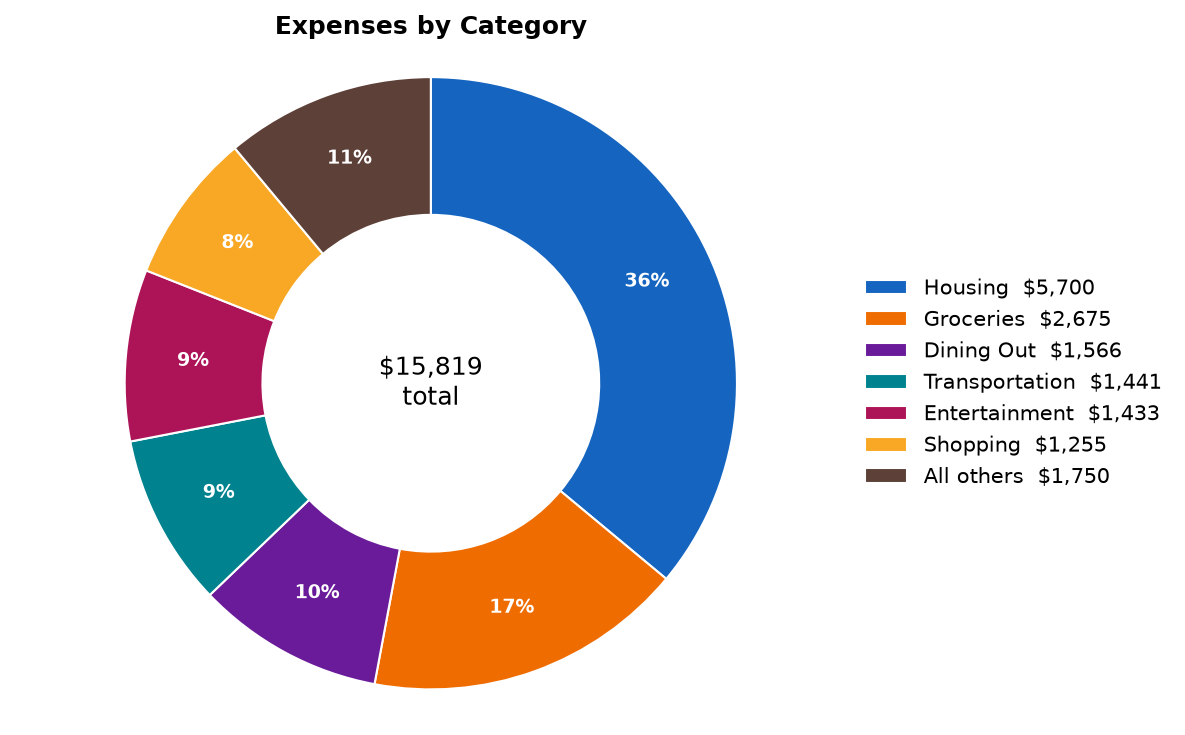
\includegraphics[width=\linewidth]{chart_category_pie.png}\end{subfigure}\hfill
  \begin{subfigure}{0.49\linewidth}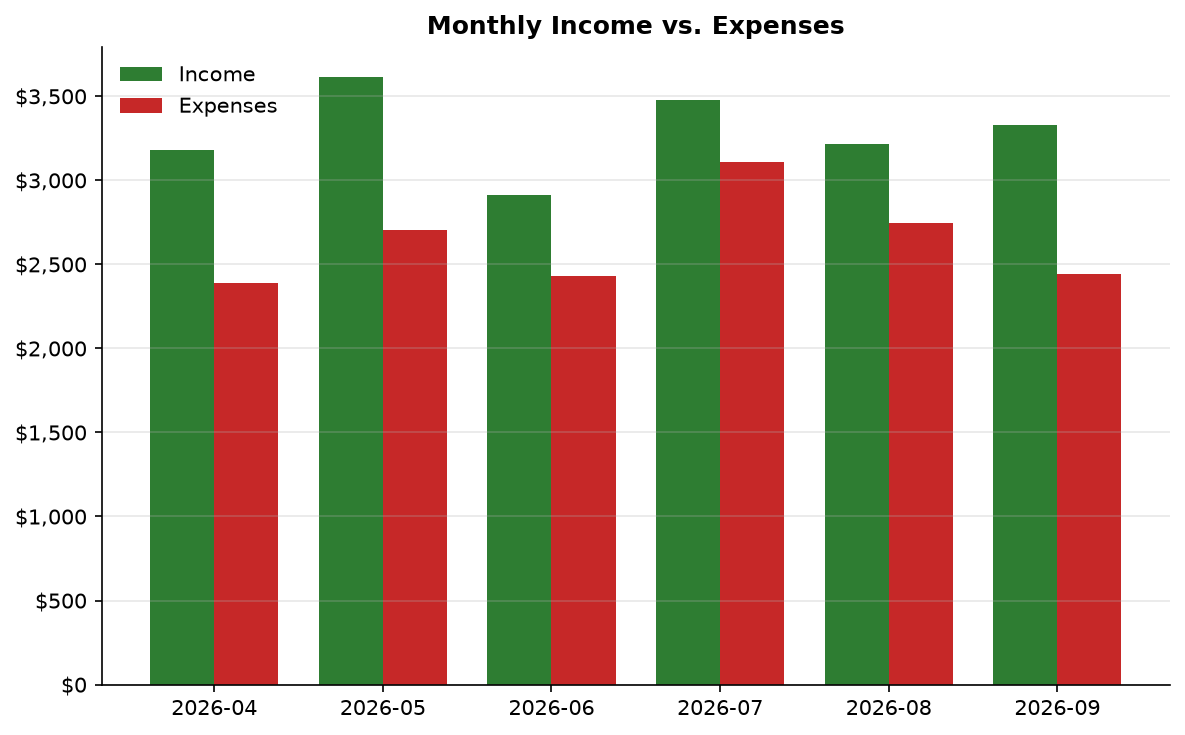
\includegraphics[width=\linewidth]{chart_monthly_income_expenses.png}\end{subfigure}

  \medskip
  \begin{subfigure}{0.49\linewidth}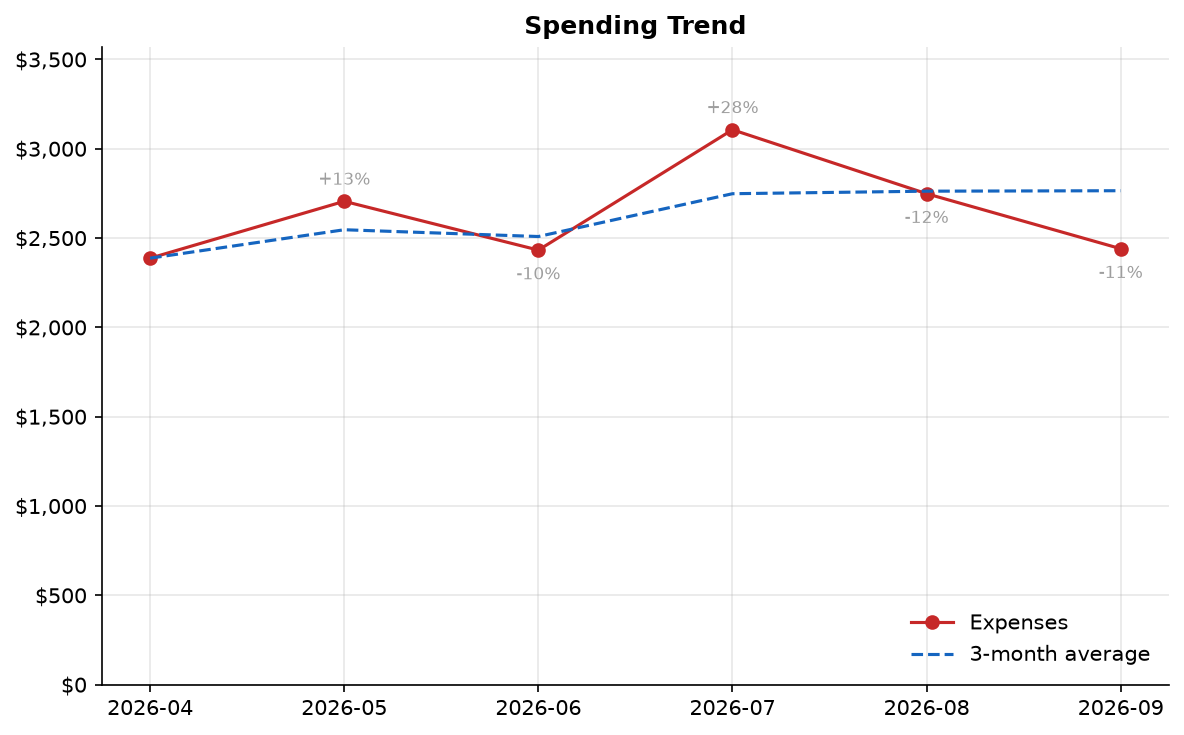
\includegraphics[width=\linewidth]{chart_spending_trend.png}\end{subfigure}\hfill
  \begin{subfigure}{0.49\linewidth}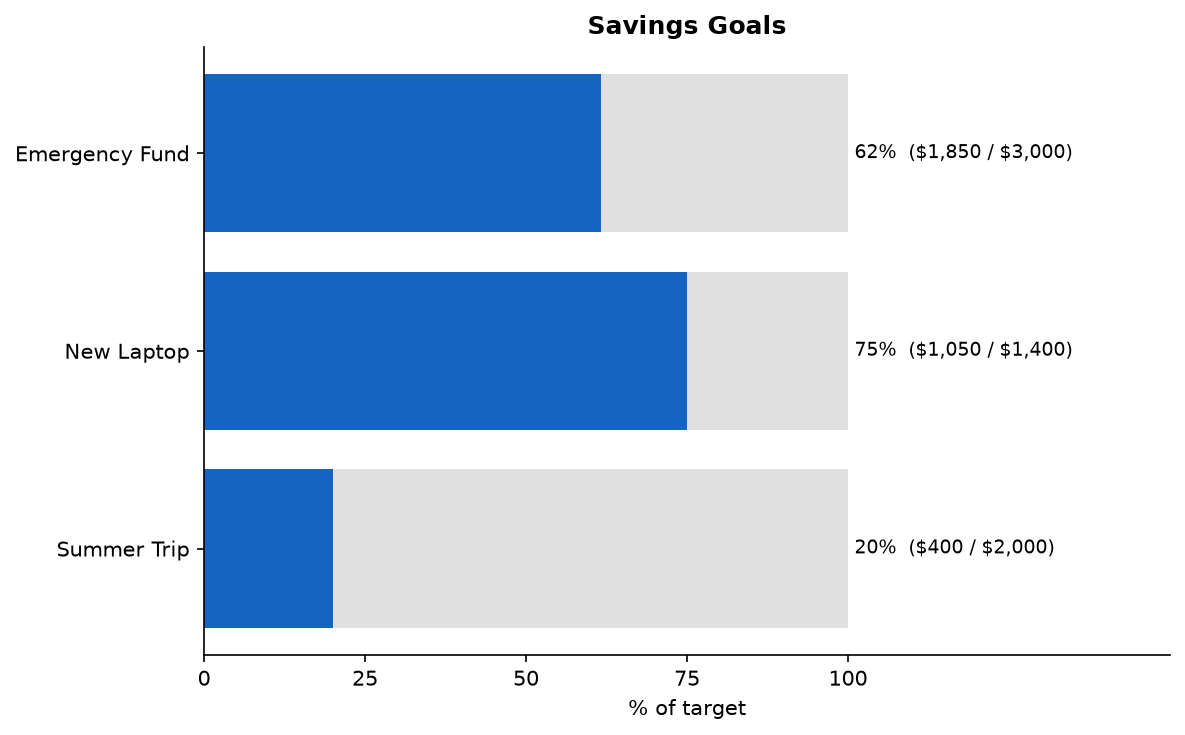
\includegraphics[width=\linewidth]{chart_goals_progress.png}\end{subfigure}
  \caption{Les quatre graphiques produits par \code{python main.py demo} dans
  \code{output/charts/} (copiés tels quels).}
  \label{figm-charts}
\end{figure}

\subsection{Plotly (\VerPlotly) et Streamlit (\VerStreamlit)}
\textbf{Rôle.} Streamlit transforme un script Python en page web ; Plotly fournit les
graphiques interactifs (survol, zoom). \textbf{Analogie.} Streamlit est une vitrine qu'on
réorganise en parlant ; Plotly, une carte qu'on peut toucher. \textbf{Où.}
\code{dashboard.py}. Le script est réexécuté de haut en bas à chaque clic ;
\code{@st.cache\_data} évite de relire le fichier si rien n'a changé.
\lstinputlisting[caption={\code{dashboard.py} --- la fonction principale de la page}]{../shared/generated/dashboard_main.py}
\textbf{Pourquoi.} Streamlit demande zéro HTML/JavaScript, contrairement à Flask ou Dash ;
Plotly est intégré nativement à Streamlit.

\subsection{Tkinter et ttk (Tk \VerTkinter)}
\textbf{Rôle.} L'application de bureau. \textbf{Analogie.} Un jeu de construction : fenêtres,
onglets, champs, boutons qu'on assemble. \textbf{Où.} \code{gui\_tkinter.py}, classe
\code{FinanceApp} (elle hérite de \code{ttk.Frame}).
\lstinputlisting[caption={\code{gui\_tkinter.py} --- le bouton \og Add transaction \fg}]{../shared/generated/gui_add_transaction.py}
\textbf{Pourquoi.} Tkinter est livré avec Python (aucune installation) et demandé par le
cours ; PyQt est plus riche mais lourd et sous licence GPL/commerciale.

\subsection{json, csv, pathlib (bibliothèque standard)}
\textbf{Rôle.} \code{json} sauvegarde tout l'état (transactions, budgets, objectifs) ;
\code{csv} échange les transactions avec Excel ; \code{pathlib} construit les chemins.
\textbf{Analogie.} JSON est un classeur avec des intercalaires ; CSV, une simple feuille de
calcul. \textbf{Où.} \code{storage.py}, \code{config.py}.
\textbf{Pourquoi.} Formats lisibles par un humain et par d'autres programmes, sans
dépendance. \code{pickle} serait illisible et dangereux à ouvrir ; SQLite serait excessif
pour quelques centaines de lignes.

\subsection{dataclasses, uuid, tempfile, argparse (bibliothèque standard)}
\code{dataclasses} génère le code répétitif des classes de données ; \code{uuid} donne à
chaque transaction un identifiant unique de 8 caractères ; \code{tempfile} et \code{os}
servent à l'écriture atomique ; \code{argparse} lit la ligne de commande
(\code{cli | gui | demo}, \code{-{}-data}, \code{-{}-output}).

\subsection{pytest (\VerPytest), pytest-cov (\VerPytestCov) et ruff (\VerRuff)}
\textbf{Rôle.} pytest lance les tests, pytest-cov mesure quelles lignes ils exécutent, ruff
vérifie et formate le style. \textbf{Analogie.} Un contrôle technique automatique avant
chaque mise en circulation. \textbf{Pourquoi.} pytest est plus concis qu'\code{unittest}
(simples \code{assert}, \emph{fixtures}) ; ruff remplace flake8, isort et black en un seul
outil très rapide.

\subsection{Outils des livrables : rich (\VerRich), Playwright (\VerPlaywright), python-docx, python-pptx}
Ils ne servent pas à l'application mais à produire les documents de façon reproductible :
rich enregistre la vraie sortie console, Playwright pilote un vrai navigateur pour capturer le
tableau de bord, python-pptx génère les slides et python-docx le document CodeStepByStep.

% ====================================================================== 4
\section{Le travail en détail, module par module}

\subsection{Vue d'ensemble et flux des données}
\begin{figure}[H]
\centering
% Architecture diagram shared by the report and the memo (TikZ).
% Requires: tikz with positioning, arrows.meta, fit, backgrounds, calc; \code macro.
\begin{tikzpicture}[
  font=\small,
  mod/.style={draw=black!55, rounded corners=2pt, fill=white, align=center,
              minimum height=9mm, text width=2.85cm, inner sep=2pt},
  file/.style={mod, fill=black!3, dashed, text width=2.85cm, font=\footnotesize},
  flow/.style={-{Stealth[length=2mm]}, thick, color=black!65},
  lbl/.style={font=\scriptsize\itshape, color=black!70, fill=white, inner sep=1pt},
  layer/.style={rounded corners=4pt, inner sep=5pt},
  x=3.75cm, y=1.9cm,
]
  % Row 1 - user interfaces
  \node[mod] (main) at (0,0)  {\code{main.py}\\cli | gui | demo};
  \node[mod] (cli)  at (1,0)  {\code{cli.py}\\console menu};
  \node[mod] (gui)  at (2,0)  {\code{gui\_tkinter.py}\\Tkinter window};
  \node[mod] (dash) at (3,0)  {\code{dashboard.py}\\Streamlit + Plotly};
  % Row 2 - application logic
  \node[mod] (alerts)    at (0,-1) {\code{alerts.py}\\80\,\% / 100\,\% rules};
  \node[mod] (tracker)   at (1,-1) {\code{tracker.py}\\FinanceTracker};
  \node[mod] (analytics) at (2,-1) {\code{analytics.py}\\pandas};
  \node[mod] (visualize) at (3,-1) {\code{visualize.py}\\matplotlib};
  % Row 3 - domain and persistence
  \node[mod] (models)     at (0,-2) {\code{models.py}\\validated dataclasses};
  \node[mod] (storage)    at (1,-2) {\code{storage.py}\\JSON + CSV};
  \node[mod] (exceptions) at (2,-2) {\code{exceptions.py}\\error classes};
  \node[mod] (config)     at (3,-2) {\code{config.py}\\pathlib paths};
  % Row 4 - files
  \node[file] (json) at (0.45,-3) {\code{data/*.json}};
  \node[file] (csv)  at (1.55,-3) {\code{data/*.csv}};
  \node[file, text width=3.3cm] (png) at (3,-3) {\code{output/charts/*.png}};

  \begin{scope}[on background layer]
    \node[layer, fill=blue!6,   fit=(main)(dash)] (L1) {};
    \node[layer, fill=green!7,  fit=(alerts)(visualize)] (L2) {};
    \node[layer, fill=orange!8, fit=(models)(config)] (L3) {};
    \node[layer, fill=violet!6, fit=(json)(png)] (L4) {};
  \end{scope}
  \foreach \l/\t in {L1/Interfaces, L2/Logic, L3/Domain, L4/Files}
    \node[font=\scriptsize\bfseries, rotate=90, anchor=south] at (\l.west) {\t};

  \draw[flow] (main) -- (cli);
  \draw[flow] (cli) -- node[lbl, right] {commands} (tracker);
  \draw[flow] (gui) -- node[lbl, left] {summaries} (analytics);
  \draw[flow] (dash) -- node[lbl, above, sloped] {filters} (analytics);
  \draw[flow] (tracker) -- (alerts);
  \draw[flow] (tracker) -- (analytics);
  \draw[flow] (analytics) -- (visualize);
  \draw[flow] (tracker) -- node[lbl, right] {save / load} (storage);
  \draw[flow] (tracker) -- (models);
  \draw[flow, {Stealth[length=2mm]}-{Stealth[length=2mm]}] (storage) -- (json);
  \draw[flow, {Stealth[length=2mm]}-{Stealth[length=2mm]}] (storage) -- (csv);
  \draw[flow] (visualize.east) -- ++(0.32,0) |- node[lbl, pos=0.25, right] {PNG} (png.east);
\end{tikzpicture}

\caption{Les modules et les flux de données. Les interfaces ne contiennent aucune règle
métier : elles envoient des commandes au \code{FinanceTracker}, qui délègue les fichiers à
\code{storage.py} ; \code{analytics} produit les DataFrames qui alimentent tableaux,
indicateurs et graphiques.}
\label{figm-archi}
\end{figure}

\Cref{figm-flow} suit le trajet d'une dépense, de la saisie à la sauvegarde.

\begin{figure}[H]
\centering
\begin{tikzpicture}[
  font=\small,
  stage/.style={draw=black!55, rounded corners=2pt, fill=white, align=center,
               text width=3.3cm, minimum height=11mm, inner sep=3pt},
  flow/.style={-{Stealth[length=2mm]}, thick, color=black!65},
  err/.style={stage, fill=red!6, draw=red!60!black, font=\footnotesize, text width=3.6cm},
  lbl/.style={font=\scriptsize\itshape, color=black!70, fill=white, inner sep=1pt},
  node distance=6mm and 5mm,
]
  \node[stage] (s1) {Saisie\\\code{prompt\_amount}, \code{prompt\_date}};
  \node[stage, right=of s1] (s2) {\code{add\_transaction}\\(FinanceTracker)};
  \node[stage, right=of s2] (s3) {\code{Transaction(\dots)}\\\code{\_\_post\_init\_\_}};
  \node[err, below=of s3] (e1) {\code{InvalidTransactionError}\\message, rien n'est gardé};
  \node[stage, below=of s2] (s4) {\code{list.append}\\\code{set.add} (catégorie)};
  \node[stage, below=of s1] (s5) {\code{check\_budgets}\\alerte 80\,\% / 100\,\%};
  \node[stage, below=of s5] (s6) {Option 0 : \code{save\_json}\\(\code{storage.py})};
  \node[stage, right=of s6] (s7) {\code{\_atomic\_write}\\fichier temporaire};
  \node[stage, right=of s7] (s8) {\code{Path.replace}\\\code{my\_finances.json}};
  \draw[flow] (s1) -- (s2);
  \draw[flow] (s2) -- (s3);
  \draw[flow] (s3) -- node[lbl, right] {invalide} (e1);
  \draw[flow] (s3.south west) -- node[lbl, above, sloped] {valide} (s4.north east);
  \draw[flow] (s4) -- (s5);
  \draw[flow] (s5) -- (s6);
  \draw[flow] (s6) -- (s7);
  \draw[flow] (s7) -- (s8);
\end{tikzpicture}
\caption{La vie d'une dépense dans le mode console : saisie validée, création de l'objet
(validation), stockage en mémoire, alerte immédiate, puis sauvegarde atomique à la sortie.}
\label{figm-flow}
\end{figure}

\subsection{\code{models.py} --- les fiches de base}
\textbf{Rôle.} Décrire une transaction, un objectif d'épargne et un budget, et refuser toute
valeur invalide. \textbf{Éléments clés.} \code{Transaction}, \code{SavingsGoal},
\code{Budget}, \code{parse\_amount}, \code{parse\_date}, \code{normalize\_category}.
\textbf{Erreurs.} Montant non numérique, nul, négatif, infini ou trop grand ; date au mauvais
format ; type autre que \code{income}/\code{expense} ; catégorie vide : chaque cas lève une
erreur précise.
\lstinputlisting[caption={\code{models.py} --- arrondir \emph{avant} de valider}]{../shared/generated/parse_amount.py}
Point fin à connaître : l'arrondi se fait \emph{avant} le test \og supérieur à zéro \fg.
Sinon \code{"0.004"} passait le test puis devenait 0,00~\$, ce qui provoquait plus tard une
division par zéro (bogue trouvé par une revue indépendante, puis corrigé et testé).

\subsection{\code{exceptions.py} --- les erreurs du projet}
\textbf{Rôle.} Donner un nom à chaque problème. \textbf{Idée clé.} L'héritage multiple :
\code{InvalidTransactionError} est à la fois une \code{FinanceTrackerError} (attrapée par
l'interface) et une \code{ValueError} (comprise par du code Python générique).

\subsection{\code{storage.py} --- lire et écrire les fichiers}
\textbf{Rôle.} Sauvegarder et charger le JSON, exporter et importer le CSV. \textbf{Éléments
clés.} \code{save\_json}, \code{load\_json}, \code{save\_csv}, \code{load\_csv},
\code{AppState}. \textbf{Gestion des erreurs.}
\begin{itemize}
  \item fichier absent : ce n'est pas une erreur (premier lancement), on part de zéro ;
  \item JSON illisible \emph{ou} mal structuré : le fichier est renommé
        \code{*.corrupted-<date>} (rien n'est perdu) et l'application démarre à vide ;
  \item enregistrement invalide ou identifiant en double : ignoré et signalé, les autres sont
        chargés ;
  \item CSV sans les colonnes obligatoires : erreur claire, avec la liste des colonnes
        manquantes.
\end{itemize}
\lstinputlisting[caption={\code{storage.py} --- \code{try / except / else} pour récupérer un fichier corrompu}]{../shared/generated/load_json.py}
\lstinputlisting[caption={\code{storage.py} --- un JSON valide mais de mauvaise forme est traité comme corrompu}]{../shared/generated/check_structure.py}

\subsection{\code{tracker.py} --- le classeur central}
\textbf{Rôle.} Contenir toutes les données en mémoire et offrir les opérations : ajouter,
modifier, supprimer, rechercher, filtrer, totaux, budgets, objectifs, import/export.
\lstinputlisting[caption={\code{tracker.py} --- ajout d'une transaction}]{../shared/generated/add_transaction.py}
\lstinputlisting[caption={\code{tracker.py} --- filtre multi-critères avec \code{continue}}]{../shared/generated/tracker_filter.py}
La modification (\code{update\_transaction}) construit un \emph{nouvel} objet : si une valeur
est invalide, l'ancienne transaction reste intacte.

\subsection{\code{analytics.py} --- les calculs pandas}
\textbf{Rôle.} Transformer la liste de transactions en DataFrame, puis calculer résumés,
répartitions, tendances et indicateurs. Chaque fonction accepte des données vides et renvoie
alors un tableau vide mais bien formé : les interfaces n'ont jamais de cas particulier.
\lstinputlisting[caption={\code{analytics.py} --- de la liste d'objets au DataFrame}]{../shared/generated/to_dataframe.py}
\lstinputlisting[caption={\code{analytics.py} --- tendance : mois continus, moyenne glissante, variation}]{../shared/generated/spending_trend.py}
Deux détails à savoir expliquer : un mois sans dépense compte pour 0 (sinon on comparerait
janvier à avril) ; une hausse depuis 0~\$ est infinie, donc affichée \og -- \fg.

\subsection{\code{alerts.py} --- budgets et jalons}
\textbf{Rôle.} Comparer les dépenses d'un mois à chaque budget, et signaler les jalons et les
échéances des objectifs. Les seuils sont des constantes (\code{WARNING\_THRESHOLD = 0.80},
\code{EXCEEDED\_THRESHOLD = 1.00}) ; les alertes sont triées de la plus grave à la moins
grave.
\lstinputlisting[caption={\code{alerts.py} --- une alerte par budget qui mérite l'attention}]{../shared/generated/check_budgets.py}

\subsection{\code{visualize.py} --- les graphiques}
\textbf{Rôle.} Quatre fonctions, une par graphique, qui renvoient une \code{Figure}.
\textbf{Pièges réglés.} Deux signes \code{\$} dans un même texte sont interprétés par
matplotlib comme une formule mathématique : ils sont échappés (\code{\textbackslash\$}). Au-delà
de 7 parts, le camembert regroupe les petites catégories dans \og All others \fg.
\lstinputlisting[caption={\code{visualize.py} --- le camembert (donut)}]{../shared/generated/category_pie.py}

\subsection{\code{config.py} --- les chemins}
Tous les chemins sont calculés à partir de l'emplacement du fichier avec \code{pathlib}
(\code{PROJECT\_ROOT}, \code{DATA\_DIR}, \code{CHARTS\_DIR}\dots) : le projet fonctionne
depuis n'importe quel dossier et sur n'importe quel système, sans chemin absolu codé en dur.

\subsection{\code{cli.py} --- le menu console}
\textbf{Rôle.} La boucle de menu et une méthode par action. \textbf{Idée clé.} Les fonctions
d'entrée et de sortie sont des paramètres (\code{input\_func}, \code{output\_func}) : les tests
pilotent des sessions entières. Ctrl+D ou Ctrl+C déclenchent une sortie propre (avec
sauvegarde), et si la sauvegarde échoue, on demande avant de quitter.
\lstinputlisting[caption={\code{cli.py} --- la boucle de menu et la dernière ligne de défense}]{../shared/generated/console_run.py}

\subsection{\code{gui\_tkinter.py} --- l'application de bureau}
\textbf{Rôle.} La classe \code{FinanceApp} construit quatre onglets, remplit les tableaux et
réagit aux clics. \textbf{Erreurs.} Toute erreur de validation s'affiche dans une boîte de
dialogue ; rien n'est enregistré. \textbf{Écrans haute résolution.} La hauteur des lignes, la
largeur des colonnes et la résolution des graphiques sont calculées à partir de la taille
réelle de la police, sinon les lignes se chevauchent.

\subsection{\code{dashboard.py} --- le tableau de bord}
\textbf{Rôle.} Barre latérale (source, période, catégories, type), indicateurs avec variation
sur le mois précédent, onglets Overview, Trends, Budgets \& Alerts, Savings Goals,
Transactions. \textbf{Erreurs.} Un fichier importé illisible affiche une erreur ; un fichier
utilisateur corrompu n'est \emph{jamais} renommé par le tableau de bord, qui ne fait que lire.
\lstinputlisting[caption={\code{dashboard.py} --- échapper \code{\$} pour le Markdown}]{../shared/generated/md_escape.py}

\subsection{\code{main.py} --- le point d'entrée}
\lstinputlisting[caption={\code{main.py} --- choisir le mode selon la ligne de commande}]{../shared/generated/main_dispatch.py}
Les imports de \code{cli} et \code{gui\_tkinter} sont faits à l'intérieur des branches : le mode
démo fonctionne même sur une machine sans Tk.

% ====================================================================== 5
\section{Les données}

\subsection{Le format CSV}
Une ligne par transaction, six colonnes ; les colonnes obligatoires sont \code{date},
\code{amount}, \code{kind} et \code{category}. Début réel de
\code{data/sample\_transactions.csv} :
\lstinputlisting[language={}, caption={\code{data/sample\_transactions.csv} (5 premières lignes)}]{../shared/generated/sample_head.csv}

\subsection{Le format JSON}
Le JSON contient tout l'état : transactions, budgets, objectifs, plus un numéro de version et
la date de sauvegarde. Extrait réel de \code{data/sample\_data.json} (2 transactions, 1 budget,
1 objectif) :
\lstinputlisting[language={}, caption={Extrait de \code{data/sample\_data.json}}]{../shared/generated/sample_excerpt.json}

\subsection{Pourquoi ces choix}
Les montants sont toujours positifs, et c'est le champ \code{kind} qui dit si c'est un revenu ou
une dépense : la validation est plus simple. Les dates sont au format ISO
(\code{AAAA-MM-JJ}), qui se trie correctement et que pandas lit directement.

\subsection{La génération des données d'exemple}
\code{tools/generate\_sample\_data.py} crée \SampleCount{} transactions \emph{fictives} sur
6 mois (\SampleFirstMonth{} à \SampleLastMonth) pour un étudiant imaginaire : salaire
toutes les deux semaines, missions freelance, loyer et abonnements fixes, dépenses variables
(courses, restaurants, transports\dots), un pic de dépenses en juillet pour rendre la tendance
intéressante, 7 budgets et 3 objectifs. Une graine aléatoire fixe (\code{42}) rend chaque
génération identique, y compris les identifiants : les tests, les captures et la vidéo
montrent toujours les mêmes chiffres.

% ====================================================================== 6
\section{Les tests}

\subsection{Ce qui est testé, et pourquoi}
Le projet compte \textbf{\TestCount{} tests automatiques}. La couverture est de
\textbf{\CoveragePct\,\%} des lignes du paquet \code{finance\_tracker}, \emph{hors}
\code{gui\_tkinter.py} et \code{dashboard.py} : ces deux fichiers sont surtout du code
d'événements graphiques, vérifié par des tests de fumée (\emph{smoke tests}).
\begin{itemize}
  \item \textbf{Modèles} : chaque règle de validation, y compris les cas limites (\code{"0.004"},
        NaN, infini, booléen, catégorie vide).
  \item \textbf{Stockage} : allers-retours JSON/CSV, fichier absent, corrompu, mal structuré,
        colonnes manquantes, lignes invalides, identifiants en double, BOM d'Excel.
  \item \textbf{Tracker, alertes, analyses} : chaque calcul pandas est comparé à un résultat
        calculé à la main sur un petit jeu de données de deux mois.
  \item \textbf{Console} : des sessions complètes pilotées par des réponses préparées, avec
        saisies invalides.
  \item \textbf{GUI et tableau de bord} : la fenêtre Tkinter est construite et cliquée sur un
        vrai affichage ; la page Streamlit tourne sans navigateur avec \code{AppTest}.
  \item \textbf{Standards} : un test vérifie les en-têtes de module, les docstrings Google, les
        annotations de type et la présence de chaque concept du cours.
\end{itemize}
\lstinputlisting[caption={\code{tests/test\_storage.py} --- un exemple de test réel}]{../shared/generated/test_corrupted_json.py}

\subsection{Comment les lancer}
\begin{lstlisting}[language=bash, caption={Lancer les tests et les contrôles de style}]
pytest -q                     # tous les tests
pytest --cov                  # avec la couverture
ruff check . && ruff format --check .
\end{lstlisting}

% ====================================================================== 7
\section{Commandes utiles}
\begin{lstlisting}[language=bash, caption={Installation (Python 3.11+ requis)}]
git clone https://github.com/14juanito/Personal-finance-tracker.git
cd Personal-finance-tracker
python3 -m venv .venv
source .venv/bin/activate          # Windows : .venv\Scripts\activate
pip install -r requirements.txt
python -m playwright install chromium   # seulement pour les captures
\end{lstlisting}
\begin{lstlisting}[language=bash, caption={Lancer l'application}]
python main.py demo                       # tout, sans interaction
python main.py cli                        # menu console
python main.py gui                        # fenêtre Tkinter
streamlit run finance_tracker/dashboard.py
\end{lstlisting}
\begin{lstlisting}[language=bash, caption={Régénérer les données et les livrables}]
python tools/generate_sample_data.py      # données d'exemple (graine 42)
python tools/capture_screenshots.py       # vraies captures -> docs/figures/
python tools/build_latex.py               # rapport + ce mémo -> deliverables/*.pdf
python tools/build_slides.py              # Demo_Slides.pptx
python tools/build_screenshot_doc.py      # document CodeStepByStep (14 captures)
python tools/build_source_zip.py          # archive du code source
\end{lstlisting}

% ====================================================================== 8
\section{Les 15 questions probables de l'évaluateur}

\newcommand{\question}[1]{\needspace{4\baselineskip}\subsection*{#1}}

\question{1. Pourquoi des dataclasses plutôt que des dictionnaires ?}
Une dataclass garantit la présence de tous les champs et permet de valider les données dans
\code{\_\_post\_init\_\_}. Elle ajoute des méthodes (\code{signed\_amount}, \code{to\_dict}).
Avec un dictionnaire, une faute de frappe dans une clé passerait inaperçue.

\question{2. Pourquoi une liste pour les transactions, mais un dictionnaire pour les budgets ?}
Les transactions ont un ordre et peuvent se ressembler : une liste convient. Un budget se
cherche par catégorie : le dictionnaire donne un accès direct et empêche d'avoir deux budgets
pour la même catégorie.

\question{3. À quoi sert l'ensemble des catégories ?}
À garantir l'unicité automatiquement. En plus, \code{normalize\_category} transforme
\og food \fg, \og Food \fg{} et \og FOOD \fg{} en \og Food \fg : ces variantes ne créent pas
trois catégories.

\question{4. Que se passe-t-il si le fichier JSON est corrompu ?}
\code{load\_json} attrape l'erreur, renomme le fichier en \code{*.corrupted-<horodatage>} (rien
n'est perdu), ajoute un avertissement et renvoie un état vide : l'application démarre
normalement. Un JSON valide mais mal structuré (\code{\{"transactions": null\}}) est traité de
la même façon. Un test le prouve :\\ \code{test\_corrupted\_json\_is\_backed\_up}
(\code{tests/test\_storage.py}).

\question{5. Et si un seul enregistrement est invalide ?}
Le chargement a un \code{try/except} \emph{par} enregistrement : la ligne fautive est ignorée et
signalée, les autres sont chargées.

\question{6. Pourquoi une écriture atomique ?}
Si le programme plante au milieu d'une sauvegarde, un fichier écrit directement serait à moitié
vide. On écrit dans un fichier temporaire, puis \code{Path.replace()} le substitue en une seule
opération. Le bloc \code{finally} supprime le fichier temporaire en cas d'erreur.

\question{7. Pourquoi JSON \emph{et} CSV ?}
Le JSON garde tout l'état, y compris les données imbriquées (budgets, objectifs). Le CSV est un
tableau plat, idéal pour Excel ou pandas, mais il ne contient que les transactions.

\question{8. Comment fonctionnent les alertes de budget ?}
Pour le mois choisi, on calcule \og dépensé / limite \fg. À partir de 0,80 c'est WARNING, à
partir de 1,00 EXCEEDED. Les alertes sont triées de la plus grave à la moins grave, et la
console comme la fenêtre en affichent une dès qu'une dépense franchit un seuil.

\question{9. Explique le résumé mensuel avec pandas.}
\code{pivot\_table(index="month", columns="kind", values="amount", aggfunc="sum")} donne une
ligne par mois et une colonne par type. On en déduit le solde et le taux d'épargne, avec une
protection contre la division par zéro quand il n'y a pas de revenu.

\question{10. Qu'est-ce que la moyenne glissante, et pourquoi l'utiliser ?}
\code{rolling(window=3).mean()} fait la moyenne des 3 derniers mois. Elle lisse un pic ponctuel
(juillet, +28\,\%) pour montrer la vraie tendance. \code{pct\_change()} donne la variation d'un
mois sur l'autre.

\question{11. Comment as-tu testé un programme interactif ?}
\code{ConsoleApp} reçoit ses fonctions d'entrée et de sortie en paramètres ; les tests lui
passent une liste de réponses et vérifient l'affichage. La fenêtre Tkinter a un test de fumée
sur un vrai affichage, et le tableau de bord est testé avec \code{AppTest} de Streamlit.

\question{12. Quel a été ton bogue le plus intéressant ?}
Les montants du type \og \$1,850 / \$3,000 \fg{} perdaient leurs signes dollar et passaient en
italique : matplotlib, comme le Markdown de Streamlit, lit le texte entre deux \code{\$} comme
une formule mathématique. Les tests ne l'ont pas vu ; c'est la capture d'écran qui l'a révélé.
Corrigé en échappant le signe, avec un test de non-régression.

\question{13. Pourquoi l'ordre des \code{except} compte-t-il ?}
\code{StorageError} hérite de \code{OSError}. Dans \code{load\_csv}, un \code{except OSError}
générique attrapait donc notre propre erreur et masquait le vrai message. Python teste les
\code{except} dans l'ordre, et un parent attrape ses enfants : on a ajouté
\code{except StorageError: raise} avant.

\question{14. Pourquoi l'interface ne contient-elle pas de logique métier ?}
Pour réutiliser et tester. Les trois interfaces appellent les mêmes fonctions : les chiffres
sont identiques partout, et la logique se teste sans écran. Ajouter le tableau de bord n'a
demandé aucune modification du cœur.

\question{15. Que pourrais-tu améliorer ?}
Des transactions récurrentes automatiques (loyer, abonnements), l'import de relevés bancaires
avec suggestion de catégorie, une base SQLite pour de gros historiques, et des prévisions de
dépenses dans le tableau de bord.

% ====================================================================== 9
\section{Glossaire}
\begin{longtable}{@{}>{\raggedright\bfseries}p{3.6cm}>{\raggedright\arraybackslash}p{11.6cm}@{}}
\toprule
\normalfont\textbf{Terme} & \textbf{Définition simple} \\
\midrule
\endhead
Agrégation & Résumer plusieurs lignes en une valeur (somme, moyenne, nombre). \\
Alerte de budget & Message affiché quand les dépenses d'une catégorie atteignent 80\,\% (WARNING) ou 100\,\% (EXCEEDED) de sa limite mensuelle. \\
Annotation de type & Indication du type attendu (\code{amount: float}), lue par les outils et les humains. \\
Atomique (écriture) & Écriture qui réussit entièrement ou pas du tout : jamais de fichier à moitié écrit. \\
Couverture de code & Pourcentage des lignes exécutées par les tests. \\
CSV & Fichier texte en tableau, une ligne par enregistrement, valeurs séparées par des virgules. \\
DataFrame & Tableau pandas : lignes, colonnes nommées, calculs vectorisés. \\
Dataclass & Classe de données dont Python écrit automatiquement le constructeur. \\
Docstring & Texte de documentation placé au début d'une fonction ou d'une classe. \\
Exception & Signal d'erreur pendant l'exécution, que l'on peut attraper avec \code{try/except}. \\
Fixture (pytest) & Donnée de test préparée une fois et fournie automatiquement aux tests. \\
\code{groupby} & Regrouper les lignes selon une colonne, puis calculer sur chaque groupe. \\
Héritage & Une classe enfant reprend tout ce que fait sa classe parente et peut l'étendre. \\
JSON & Format texte de données structurées (objets, listes), lisible par l'humain. \\
Moyenne glissante & Moyenne recalculée sur une fenêtre qui avance (ici 3 mois). \\
\code{pathlib} & Module standard qui manipule les chemins de fichiers comme des objets. \\
\code{pivot\_table} & Tableau croisé : lignes, colonnes et valeur agrégée choisies. \\
Pseudo-terminal & Terminal simulé ; sert à enregistrer une vraie session console. \\
Smoke test & Test rapide qui vérifie qu'une interface démarre et réagit, sans tout détailler. \\
Taux d'épargne & (revenus $-$ dépenses) $/$ revenus, en pourcentage. \\
Tkinter / ttk & Bibliothèque graphique livrée avec Python ; ttk fournit des widgets modernes. \\
Treeview & Widget Tkinter qui affiche un tableau à colonnes. \\
Validation & Vérifier qu'une donnée est correcte avant de l'accepter. \\
Xvfb & Écran virtuel sous Linux, utilisé pour capturer la fenêtre sans afficher l'écran réel. \\
\bottomrule
\end{longtable}

\end{document}
